\edef\mychapter{Set Theory}
\edef\mychapterdate{June 18, 2024}

\chapter{\mychapter}
Moving from logic to some more recognizable mathematics, we will first introduce the concept of a set.
We will split the section into two parts: one dedicated to na\"ive set theory, and an introduction to more formal set theory.
For mathematicians, na\"ive set theory is sufficient to make sense of most mathematical concepts, but as it turns out, formalizing set theory gives us a concrete way to trace back complicated concepts like infinity to relatively simple ones like first-order logic.
I will try to give a sneak peek to the reader of this prospect at the end of this chapter.

\section{Set Theory Basics}
For now, we will begin by giving an informal definition of sets to explore the basic ways that these mathematical objects interact.
As we should have already seen in the previous chapter, the idea of a \textit{set} or \textit{collection} arises very naturally in mathematics and logic.
For this reason, many regard the set as the most fundamental concept in all mathematics.

At the most foundational level, a \textit{set} is a mathematical object that contains other mathematical objects.
Now, although most sets of students encounter in high school math consist of just numbers, this doesn't necessarily have to case; in fact, sets can contain anything from functions, matrices, equations, or even sets themselves.\footnote{
I should note here that this idea of self-containment can be a source of great contradiction if not correctly managed. We will demonstrate this when we introduce set theory from a more formal approach.}

A convention that many mathematicians imply is to denote sets with \textit{capital letters}, so using this convention, we can give the following examples of sets
\begin{equation}
	A = \{1, a, b\},
\end{equation}
\begin{equation}
	B = \{f(x)=x^2+2, g(x)=3x+2, +\footnotemark\},
\end{equation}
\footnotetext{The \textit{plus} sign is \textit{technically} a mathematical object (more specifically a function of two variables), thus, there is nothing wrong with including it in a set.}
where the elements of the sets are denoted between the curly braces.

Now, I've given examples of \textit{finite sets}, but as we will see, \textit{finiteness} is certainly \textit{not} a requirement for a collection to be a set.

\subsection{Notation}
To make talking about sets easier, we will introduce the following notion as seen in \cref{fig:set-notation}.
\begin{figure*}[h]
	\centering
	\begin{tabular}{| c | m{6cm} |}
		\hline
		Symbol & Meaning \\
		\hline
		$\in,\notin$   & in and not in, respectively	\\
		\hline
		$\subset, \subseteq$ & proper subset, subset \\
		\hline
		$\not\subset, \not\subseteq$ & negations of above\\
		\hline
		$=$ & equivalent \\
		\hline
		$\cup$ & Union \\
		\hline
		$\cap$ & Intersect \\
		\hline
		$A^c$ & Compliment of $A$\\
		\hline
		$\setminus$ & Set difference \\
		\hline
		$\varnothing$ & Empty set, a set with no elements.\footnotemark\\
		\hline
	\end{tabular}
	\caption{}
	\label{fig:set-notation}
\end{figure*}
\footnotetext{Some texts commonly use the term \textit{null set} for an empty set, but the term \textit{null set} is also commonly used in math to refer to something completely different, so we will be solely using the term \textit{empty set} in this text.}

These symbols can be broken down into two main categories: The relational operators and the logical operators.
We will discuss them separately, but we will start with the relation operators.

The relational operators denote relationships between sets and can be understood by the direct English translations.
Many times, math symbols are created to shorthand English words, and as such, a way to understand and unravel the meaning behind these symbols is to translate them to the specific English words that they represent.

For example, we can interpret the phrase $x\in X$ to be \textit{$x$ in $X$} or \textit{$x$ is an element of $X$}.
By adding a slash through it, $x\notin X$ becomes the negation of the above, hence we have \textit{$x$ is not in $X$}.

Similarly, $X\subseteq Y$ and $X\not\subseteq Y$ can be understood as
\textit{$X$ is a subset of $Y$} and \textit{$X$ is not a subset of $Y$} respectively.
A set is a subset of a larger set if all of its components are included within the larger set, as seen in \cref{fig:subset}.
\begin{figure}[h]
	\centering
	\resizebox{0.3\linewidth}{!}{
	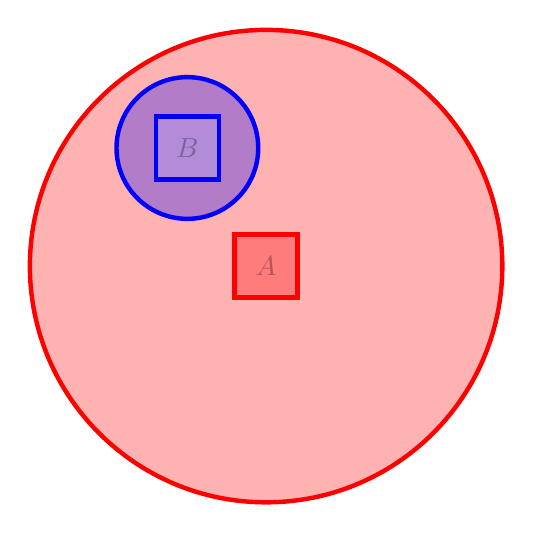
\begin{tikzpicture}
		\draw[ultra thick, draw=red, fill=red, fill opacity=.3] (0,0) circle (3)
			node[black,draw=red, fill=red, minimum size=0.8cm] {$A$};
		\draw[ultra thick, draw=blue, fill=blue, fill opacity=.3] (-1,1.5) circle (0.9)
			node[black,draw=blue, fill=blue!30, minimum size=0.8cm] {$B$};
	\end{tikzpicture}}
	\caption{Here we claim $B\subset A$}
	\label{fig:subset}
\end{figure}

Like how the $=$ is normally used in math, $A=B$ implies $A$ and $B$ are the same set.

Apart from $\in, \notin$, we can also give formal definitions of these symbols, shown as follows

\begin{define}
	$A\subseteq B$ if and only if for every $a\in A$, $a\in B$

	Similarly, $A\not\subseteq B$ if and only if there exists $a\in A$ such that $a\notin B$.
\end{define}

Notice, with these definitions, $A\subseteq A$ is a true statement, meaning a set is always a subset of itself.
Sometimes, to clarify that a subset is strictly smaller than the parent, we introduce the symbols $\subset$ and $\not\subset$ to denote \textit{proper subset} and \textit{not a proper subset} respectively.
A proper subset differs from a normal subset in the fact that proper subsets must not be equal to their parent; hence, we can give the following definitions:

\begin{define}
	$A \subset B$ if and only if $A\subseteq B$ and $A\neq B$.

	$A \not\subset B$ if and only if $A\not\subseteq B$ or $A\neq B$.
\end{define}

It turns out, when defining the \textit{equality} operator, we can characterize these using the subset operators.
To claim that two sets are equal is to claim that any element in either set is also in the other.
In other words,
\begin{equation}
	x\in A \text{ if and only if } x \in B.
\end{equation}
One can check that this characterization is equivalent to
\begin{equation}
	A\subseteq B \text{ and } B\subseteq A.
\end{equation}
Using this characterization, one arrives at the following:
\begin{define}
	$A=B$ if and only if $A\subseteq B$ and $B\subseteq A$.
\end{define}

Now, we can move on to the logical operators of set theory.
As one might expect, these operators are very much related to the logical operators that we saw in the previous chapter.
Unlike the relational operators, logical operators give a means to generate new sets, much like how addition and subtraction operators work with traditional arithmetic.

We start with \textit{union} and \textit{intersection} operators, which are the set-theoretic disjunction and conjunction operators.
As such, we can give the following definitions:
\begin{define}
	Let $A$ and $B$ be arbitrary sets, then $x\in A\cup B$ if and only if $x\in A$ or $x\in B$.
	\label{def:union}
\end{define}
\begin{define}
	Let $A$ and $B$ be arbitrary sets, then $x\in A\cap B$ if and only if $x\in A$ and $x\in B$.
	\label{def:intersect}
\end{define}

\cref{fig:union} shows the intersection and union operators as a Venn diagram, where the entire Venn diagram represents the union of $A$ and $B$.
\begin{figure}[h]
\centering
\resizebox{0.6\linewidth}{!}{
	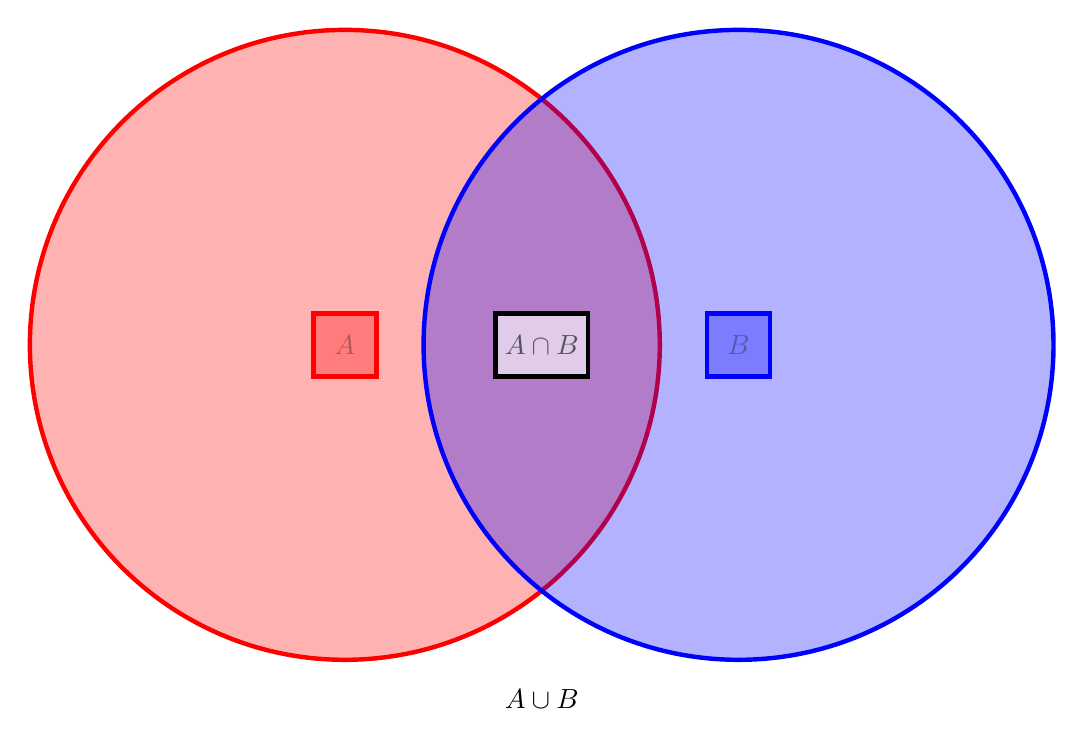
\begin{tikzpicture}
		\draw[ultra thick, draw=red, fill=red, fill opacity=.3] (-2.5,0) circle (4) node[black,draw=red, fill=red, minimum size=0.8cm] {$A$};
		\draw[ultra thick, draw=blue, fill=blue, fill opacity=.3] ( 2.5,0) circle (4) node[black, draw=blue, fill=blue, minimum size=0.8cm] {$B$};

		\draw (0,0) node[ultra thick, draw=black, fill=white, minimum size=0.8cm, fill opacity=0.6] {$A\cap B$} ;

		\draw (0,-4.5) node {$A\cup B$} ;
	\end{tikzpicture}}
	\caption{}
	\label{fig:union}
\end{figure}

Similarly, \textit{set complements} are the set-theoretic negation operator.
Its definition is given as follows:
\begin{define}
	Let $A$ be a set. Then $x\in A^c$ if and only if $x\notin A$.
\end{define}

\cref{fig:not} shows the complement as an operator.
\begin{figure}[h]
\centering
	\resizebox{0.3\linewidth}{!}{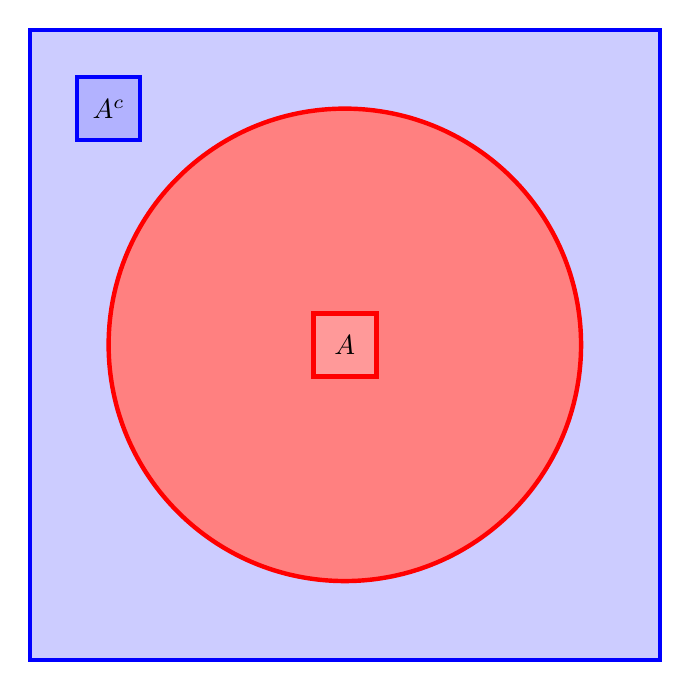
\begin{tikzpicture}
		\draw[ultra thick, draw=blue, fill=blue, fill opacity=.2] (-4,-4) rectangle (4,4);
		\draw[ultra thick, draw=red, fill=red!50] (0,0) circle (3) node[black,draw=red, fill=red!40, minimum size=0.8cm] {$A$};
		\draw (-3,3) node[ultra thick, black, draw=blue, fill=blue!30, minimum size=0.8cm] {$A^c$};
	\end{tikzpicture}}
	\caption{}
	\label{fig:not}
\end{figure}
It should be noted that the complement operator usually requires some assumption of a universal set.
In \cref{fig:not}, the universal set can be represented by the entire area enclosed by the outer blue square.
In most cases, this universal set can be easily identified, but in certain cases where we'd like to specify the universal set in question, we can utilize the \textit{set difference} operator.

When we write $A \setminus B$, the resulting set is the complement in $B$ that is fully contained in $A$.
As such, the definition, very similar to the complement operator, is given as
\begin{define}
	Let $A$ and $B$ be arbitrary sets.
	Then $x\in A\setminus B$ if and only if $x\in A$ and $x\notin B$.\footnotemark
\end{define}
\footnotetext{
	Notice we didn't require $B \subseteq A$.
	This is to means $A\setminus B$ is still a valid statement even if $B$ is entirely not contained in $A$.
	In the cases where $A$ and $B$ are mutually disjoint ($A\cap B=\varnothing$), $A\setminus B = A$.
}

As seen in \cref{fig:set-minus}, the area shaded in red not covered by the blue circle is the result of $A \setminus B$.
\begin{figure}[h]
\centering
\resizebox{0.3\linewidth}{!}{
	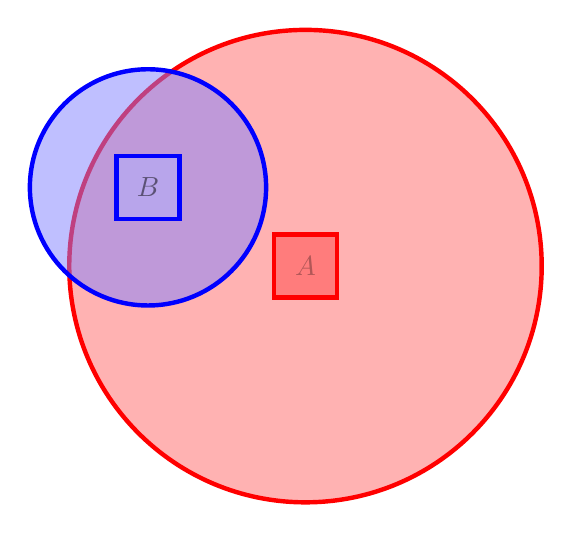
\begin{tikzpicture}
		\draw[ultra thick, draw=red, fill=red, fill opacity=.3] (0,0) circle (3)
			node[black,draw=red, fill=red, minimum size=0.8cm] {$A$};
		\draw[ultra thick, draw=blue, fill=blue!50, fill opacity=0.5] (-2,1) circle (1.5)
			node[black,draw=blue, fill=blue!30, minimum size=0.8cm] {$B$};
	\end{tikzpicture}}
	\caption{$A\setminus B$ defined in red}
	\label{fig:set-minus}
\end{figure}

\subsection{Set Building}
Now that we have a means of talking about and manipulating sets, in this next section, we shall look at examples of sets and ways to construct sets from sets that we already have.

To begin, I've listed in \cref{fig:important-sets} many important sets that we commonly encounter in math.
\begin{figure}[h] \label{fig:important-sets}
	\centering
	\begin{tabular}{| c | m{6cm} |}
		\hline
		Symbol & Definition \\
		\hline
		$\integ$ & Set of all integers \\
		\hline
		$\nat$ & Set of all natural numbers \\
		\hline
		$\real$ & Set of all real numbers \\
		\hline
		$\complex$ & Set of all complex numbers \\
		\hline
		$\rat$ & Set of all rational numbers \\
		\hline
	\end{tabular}
	\caption{}
\end{figure}

The set of integers is the set of all whole numbers (both positive and negative), as many of you hopefully will have seen in previous math classes.
The natural numbers are simply a subset of the integers that consists of only positive (non-zero) integers (e.g 1,2,3,...).\footnote{
	Depending on whom you ask, some people also consider the number 0 a natural number.
	However, as we will find out, this doesn't really change anything (in terms of the structure of the set) and just impacts how we choose to interpret this set.
	In fact, the structure of $\nat$ remains unchanged regardless of where you decide to start it (i.e. taking $\nat$ to be the set of all integers greater than -1,000 would still be equivalent to the standard definition of $\nat$ in the eyes of a set theorist in some sense.)}
We will discuss the rational numbers later on in this section; real and complex numbers in another chapter.

To construct subsets of any existing set, mathematicians commonly employ what is known as a \textit{set-builder}.
As with most other mathematical notation, the symbol we will introduce has very nice translations into English.

Let's say we want to define $A$ as a subset of the integers such that every element is even. We can write
\begin{equation}
	A=\{x\in \integ \mid \textit{x is even}\}
	\label{eq:sample-set-build}
\end{equation}
where $\mid$ translates to the word \textit{given} or \textit{provided}.
Translating equation \eqref{eq:sample-set-build}, we have
\begin{equation}
	A \text{ is equivalent to a set where } x\in \integ \text{ is an element } \textit{provided } x \text{ is even}.
\end{equation}

Often, if the set that we are taking a subset from can be easily inferred, we commonly shorthand equation \eqref{eq:sample-set-build} to
\begin{equation}
	A=\{x \mid \textit{x is even}\}.\footnotemark
\end{equation}
\footnotetext{
	With a bit more mathematical wizardry, we can make this definition of even integers a bit more sophisticated in the following way:
	$$A=\{x \mid (\exists n \in \integ)(x=2n)\}.$$
}

Although originally designed for taking subsets, this notation is sometimes abused to construct sets like the \textit{power set}.
The power set is a powerful tool in set theory, most notably used in the creation of larger sets.
The power set of any set, denoted by $P(A)$, is the set of all subsets of any given set.
Abusing the notation we developed before, we can define
\begin{equation}
	P(A):=\{U \mid U \subseteq A\}.
\end{equation}
Notice, besides the power set itself, there is no set containing all the subsets of $A$ from which we can take $P(A)$ to be a subset of.\footnote{This abuse of notation is commonly what we use to define a class, which is the same as a set in many but certainly not all cases.
We will discuss the differences when we take a more rigorous approach to set theory.}
%TODO: add definition of := somewhere

If we let $(x,y):=\{x,\{y\}\}$,\footnote{When we define sets more rigorously, we want every object we work with to be a \textit{set}, hence the weird definition of an ordered pair.} we can also define the set of all \textit{ordered pairs} as a set of sets, where if $X$ and $Y$ are sets, then
\begin{equation}
	X\times Y := \{(x,y) \mid x \in X \text{ and } y \in Y\}.
\end{equation}
where $(x,y)$ is the set defined above and $X\times Y$ is the \textit{cartesian product} of $X$ and $Y$, or the set of all ordered pairs of elements in $X$ followed by elements in $Y$.

We can, in theory, repeat the process of taking Cartesian products to get sets of ordered triples, quadruples, or more generally, ordered \textit{$n$-tuples}.
As $n$ gets large, to help facilitate with notation, let $\mathcal C$ be a collection of sets.
Then to take an $n$ product of sets in $\mathcal C$, we first assign each natural number $i \le n$ to a unique element in $\mathcal C$.
This makes precise the statement \textit{$i$th set in $\mathcal C$}, which we take to mean the element $C_i\in mathcal C$ with the index $i$.
With this, we can denote the $n$-product as
\begin{equation}
	\prod_{C_i \in \mathcal C} C_i := C_1 \times C_2 \times ... \times C_n.
\end{equation}
To denote each $n$-tuple we write $(c_i)_{i\le n}$, were each $c_i\in C_i$ is the $i$th element in the tuple.

Note, we might have $C_m=C_n$ for $m\neq n$, for example, if we take the product of $n$ copies of $C$, then the collection $\mathcal C$ has one element and $C_i=C_j$ for all $i,j \le n$.
Thus, this product
\begin{equation}
	\underbrace{C \times ... \times C}_n = \prod_{i \le n} C_i
\end{equation}
If the product consists of a single set, sometimes, we simplify the notation by simply writing $\prod_{i\le n} C$, or $C^n$.

To generalize this to infinite products, observe in the finite case, if we let $I$ be the collection of indices, $I$ is the set
\begin{equation}
	I:=\{k \in \nat \mid k \le n\}.
\end{equation}
To generalize to infinite products, we simply allow this indexing set $I$ be arbitrary.
Then like before, if we assign each element $i \in I$ to a unique element in $\mathcal C$, we denote the product $\prod_{i \in I} C_i$ as the set of infinite tuples $(c_i)_{i \in I}$ where $c_i \in C_i$ for each $i \in I$.
In general, we will refer infinite tuples as simply a \textit{sequence} when we take the indexing set to be $\nat$.\footnote{We will see that infinite indexing sets are not all created equal: in particular a collection indexed by $\real$ results in a significantly different product than a collection indexed by $\nat$. We will see the reasons for why in a later section.}
Like in the finite case, when we take the infinite product of the same set, we denote this product as $C^I$ where, $I$ is the indexing set.

Let's also denote a very special type of set by the following definition:
\begin{define} \label{def:singleton}
	Let a \textit{singleton} denote any one-point-set (i.e. sets of the form $\{x\}$).
\end{define}

\section{Relations}
Relationships are one of the most important constructions in all math, and in this section, we will develop strategies for dealing with them, along with different ways they can be helpful in our mathematical toolbox.
We will mostly be focusing on \textit{binary relations} (relations between two objects), but similar constructions as seen in this chapter can be used to understand any n-relation.

To start, let's provide ourselves with a set-theoretic definition of a relation:
\begin{define}
	Let $\square\subseteq X \times Y$ be a binary relation.
	Then we say $x \,\square\, y$\footnotemark if and only if $(x,y)\in \square$.\footnotemark
	\label{def:bin-rel}
\end{define}
\addtocounter{footnote}{-1}
\footnotetext{$x$ is related to $y$ by $\square$}
\addtocounter{footnote}{1}
\footnotetext{I will note that this definition of a relation is only here to make the relation itself a set.
As noted in a previous footnote, this is advantageous when we define sets rigorously so that every object we work with is a set, but unnecessary for a proper understanding of relations in general.
The remaining concepts developed in this chapter are independent of whether you take the relation to be set-theoretic or not.
}

\begin{ex}
	To explain how this works, we will use an example of a relation and build the set-theoretic version of this.
	This relation I shall choose is $\le$, as defined for integers, since most of our readers should be familiar with it.
	To separate this relation from the set-theoretic relation, I will use $\triangle$ for the set-theoretic relation that we will define based on $\le$.

	First, to establish the sets we are relating, we will define
\begin{equation}
	S:=\{n\in\nat : n \le 3\}
\end{equation}
to be used as both operands.
Thus, $\triangle \subseteq S^2$.\footnote{$S^2=S\times S$}

Then by the \cref{def:bin-rel}, so that $\triangle$ is a representation of $\le$, we require
\begin{equation}
	\triangle = \{(s,t)\in S^2 \mid s \le t\},
\end{equation}
thus
\begin{equation}
	\triangle=\{(1,1),(1,2),(1,3),(2,2),(2,3),(3,3)\}.
\end{equation}
One can check by definition of the set-builder, for $s,t\in S$, $s\triangle t$ (implying $(s,t) \in S^2$) if and only if $s\le t$.
\end{ex}

\subsection{Equivalence Relations}
Now, a binary relation is too broad a concept to really have interesting properties on its own, so for the remaining part of this chapter, we will restrict our attention to specific types of relations.
First, we will turn our attention to the concept of an equivalence relation.

\begin{define}
	Let $S$ be a set and $\sim\subseteq S^2$ be a relation.
	$\sim$ is an equivalence relation if the following hold:
	\begin{enumerate}[label=(A\arabic*)]
		\item (reflexive)  $x \sim x$,
		\item (symmetric) $x \sim y$ implies $y \sim x$,
		\item (transitive) $x\sim y$ and $y\sim z$ implies $x\sim z$.
	\end{enumerate}
\end{define}

As we can see, the equality relation, whether in numbers or in sets, satisfies all the axioms to be an equivalence relation.
But as we will find out, equivalence relations can describe a far more general class of relations that resemble equivalence.

\begin{ex}
	To show an example of an equivalence relation, let's define a set
	\begin{equation}
		S:=\{a,b,c, 1,2,3,\alpha,\beta,\gamma\}.
	\end{equation}
	Using this set, we will define a relation where only characters of the same type are related to each other, hence $a\sim b$, $\alpha\sim \beta$, but $1 \not\sim a$.
	One can easily check that every property of an equivalence relation holds; hence, this is an equivalence relation.

	We can also define for each element $s\in S$,
	\begin{equation}
		[s]_\sim:=\{t \in S \mid s \sim t\}
	\end{equation}
	which we shall name an \textit{equivalence class}.
	Then notice
	\begin{align}
		&[a]_\sim=[b]_\sim=[c]_\sim=\{a,b,c\} \\
		&[1]_\sim=[2]_\sim=[3]_\sim=\{1,2,3\} \\
		&[\alpha]_\sim=[\beta]_\sim=[\gamma]_\sim=\{\alpha,\beta,\gamma\}.
	\end{align}
	A notable observation is that these equivalence classes partition $S$ into three sets, which are completely disjoint when not equivalent.
	In addition, $s\in [s]$ by the reflexive property and $[s]=[t]$ is equivalent to writing $s\sim t$.
	\label{ex:eq-rel}
\end{ex}

Now, the idea that an equivalence relation can partition a larger set into distinct classes applies far more generally than what is seen in \cref{ex:eq-rel}.
This is, in fact, what makes these relations "equivalent" as relations between elements exactly correspond to the equivalence of equivalence classes.
We will formalize everything with these theorems:

\begin{thm}
	Let $S$ be a set and $\sim$ be an equivalence relation on $S$.
	Then for any $s,t\in S$, $s\sim t$ if and only if $[s]=[t]$.
	\label{thm:equ-rel-equ}
\end{thm}
\begin{proof}
	Suppose $s\sim t$. Let $u\in [s]_\sim$, then $s\sim u$ by definition.
	By the symmetric property, we have $t \sim s$, hence by transitivity, $t \sim u$.
	Therefore, $u\in [t]_\sim$ by definition.
	Thus, $[s]_\sim\subseteq [t]_\sim$.

	Using a similar process, we also obtain $[t]_\sim \subseteq [s]_\sim$ thereby proving $[s]_\sim=[t]_\sim$.

	Conversely, suppose $[s]=[t]$, then $t\in [s]$, thus $s\sim t$ by definition.
\end{proof}

\begin{thm}
	Let $S$ be a set and $\sim$ be an equivalence relation on $S$.
	Then the equivalence classes of $\sim$ partitions $S$.
	\label{thm:equ-rel-part}
\end{thm}
\begin{proof}
	We first need to show that the equivalence classes cover the entire set $S$.
	This is trivial since one could check
	\begin{equation}
		\bigcup_{s\in S} [s]_\sim = S.\footnotemark
	\end{equation}
	\footnotetext{This notation means $[s_1]_\sim \bigcup [s_2]_\sim \bigcup ...$ for $s_1, s_2, ...$ are distinct elements in $S$.}

	Next, we will show that distinct equivalence classes are disjoint, or in other words, $[s]_\sim\cap [t]_\sim \neq \varnothing$ implies $[s]_\sim=[t]_\sim$.
	If $[s]_\sim \cap [t] \neq \varnothing$, then let $u \in [s]_\sim \cap [t]_\sim$.
	By definition of $u\in [s]_\sim$ and $u\in [t]_\sim$, we have $s\sim u$ and $t\sim u$.
	Using the symmetric followed by the transitive property of the equivalence relations, we obtain $s\sim t$, whereby \cref{thm:equ-rel-equ} we conclude $[s]_\sim = [t]_\sim$.
\end{proof}

\subsection{Ordering Relations}
Next, what we will consider are relations that denote order.
Actually, what we will come to realize is that ordering relations are just slightly weaker versions of equivalence relations.

We will first direct our attention to a slightly weaker version of an order, also known as a \textit{partial order}.
Even though we will use the symbol $\le$, a partial ordering is still too weak to really resemble any standard ordering you might have seen in the past; however, this is the convention, so we will stick with it.

\begin{define}
	Let $P$ be a set. $\le$ is \textit{partial ordering} if the following are true:
	\begin{enumerate}[label=(A\arabic*)]
		\item (reflexive)  $x \le x$,
		\item (antisymmetric) $x \le y$ and $y \le x$, then $x=y$,
		\item (transitive) $x\le y$ and $y\le z$ implies $x\le z$,
	\end{enumerate}
	for all $x,y,z \in P$.
\end{define}

A set $P$ equipped with an order relation $\le$ are often denoted together by the ordered pair $(P,\le)$ and is commonly referred to as a \textit{poset}.

\begin{ex} \label{ex:power-poset}
	Let $X$ be an arbitrary set.
	We show that the power set $P(X)$ can be partially ordered by the subset relation, thus making $(P(X),\subseteq)$ a poset.

	We can first check that $\subseteq$ is reflexive since for every $S\in P(X)$, $S\subseteq S$.
	The antisymmetric property is satisfied by the definition of equality for sets, namely, $S \subseteq T$ and $T\subseteq S$ if and only if $S=T$ for arbitrary sets.
	Finally, one could quickly check by the definition of subset, $S\subseteq T$ and $T\subseteq U$ implies $S \subseteq U$ (see \cref{exer:subset-trans})
\end{ex}

\begin{define}
	Let $X$ be a poset.
	\begin{enumerate}
		\item $a$ is the \textit{greatest element} if and only if for every $x\in X$, $x \le a$.
		\item $a$ is the \textit{least element} if and only if for every $x\in X$, $a \le x$.
		\item $a$ is a \textit{maximal element} if and only if for every $x\in X$, $x=a$ or $a \not\le x$
		\item $a$ is a \textit{minimal element} if and only if for every $x\in X$, $x=a$ or $x \not\le a$.
	\end{enumerate}
\end{define}

The greatest elements are not the same as the maximal, and while greatest elements are necessarily unique, maximal elements are not.
Similarly, the same can be said about the minimal and least elements.

\begin{ex}
	%TODO: add example for maximal and least elements.
\end{ex}

While powerful, posets are of limited use for the math developed in this book, so to make this concept more useful, we will impose stronger conditions.
Observe in \cref{ex:power-poset}, we can construct $X=\{1,2,3\}$ and $S=\{1\}$ and $T=\{2\}$.
It follows that $S\not \subseteq T$ and $T\not \subseteq S$.
As one can see, for a partial ordering, not every element is comparable, which sharply contrasts with what we see with any standard ordering of numbers.
For this reason, any sets ordered by a partial ordering can't be represented in a line (in general), like what we see with a number.
Instead, posets are more generally represented by a graph,\footnote{
	The \textit{graph} seen here is not the \textit{plot} of a function but rather a collection of nodes called \textit{vertices} connected by lines called \textit{edges}.
	In this book, \textit{plots} of functions will be referred to as such to minimize confusion.}
as seen in \cref{fig:poset-graph}.

\begin{figure} \caption{} \label{fig:poset-graph}
	%TODO: add poset graph
\end{figure}

To make an ordering fit on a line, we will introduce a \textit{linear ordering} or a \textit{total ordering} defined as follows:

\begin{define}
	Let $X$ be a set.
	Then $X$ is a \textit{linear ordering} if the following hold:
	\begin{enumerate}[label=(A\arabic*)]
		\item (reflexive)  $x \le x$,
		\item (antisymmetric) $x \le y$ and $y \le x$, then $x=y$,
		\item (transitive) $x\le y$ and $y\le z$ implies $x\le z$,
		\item (totality) $x\le y$ or $y \le x$.
	\end{enumerate}
	for all $x,y,z \in P$.
\end{define}

As one should notice, all linearly ordered sets are posets, and I will leave it to the reader that orderings of numbers like integers, rationals, or real numbers are linearly ordered.

We, in particular, will be interested in a specific type of linear ordering, namely a \textit{well-ordering} which we define here:

\begin{define}
	Let $X$ be a set with a linear ordering by $\le$.
	$X$ is \textit{well-ordered} by $\le$ if and only if every subset of $X$ has a least element.
\end{define}

For any finite subset of a linearly ordered set, one can easily find the least element by comparing each element one by one.
Since every subset of a finite set is finite, we have the following result:

\begin{prop} \label{prop:finite-linear-order}
	Let $F$ be finite linearly ordered set. Then $W$ is well-ordered.
\end{prop}

Perhaps a more interesting result is the fact that $\nat$ is well-ordered.
Since not every subset of $\nat$ is finite, the method of comparing each element one by one no longer holds.
Thus, let me provide another way one might prove this fact.

\begin{thm}
	$\nat$ is well-ordered.
\end{thm}
\begin{proof}
	Let's begin by defining our $n$-sets as
	\begin{equation}
		N_n = \{k\in \nat \mid k \le n\}.
	\end{equation}
	One can easily check the set of $n$-sets is linearly ordered by $\subseteq$ and in particular,
	\begin{equation} \label{eq:order-preservation-N_n}
		N_n \subseteq N_m \iff n \le m.
	\end{equation}
	Given any subset on $\nat$, we can represent each element uniquely as an $n$-set and by equation \eqref{eq:order-preservation-N_n}, the order passes nicely between the two representations.
	Thus, for any $S\subseteq$, we can reduce the problem of finding the least element of $S$ to finding the least element of $\mathcal S :=\{N_n \mid n \in S\}$.

	First, let's consider the intersection of $\mathcal S$, which we denote as $\bigcap_{n \in S} N_n$.
	We show this forms an $n$-set.
	Since for each $N_k \in \mathcal S$, $\bigcap_{n \in S} N_n \subseteq N_k$, the intersection is finite thus one can find its maximum, which we denote as $n_M$.
	In particular, since $n_M \in N_k$ for each $N_k \in \mathcal S$ by the intersection, we require that for every $l \le n_M$, $l \in N_k$ for each $N_k$ by the definition of $n$-sets.
	Therefore, we conclude
	\begin{equation}
		N_{n_M} = \bigcap_{k \in S} N_k.
	\end{equation}

	Since $N_{n_M} \subseteq N_k$ for each $N_k$, if we show $N_{n_M} \in \mathcal S$, then $N_{n_M}$ is the least element of $\mathcal S$ and thus $n_M$ is the least element of $\mathcal S$.
	We show this by assuming the converse.
	Thus, $N_{n_M} \subsetneq N_k$ which implies $n_M+1 \in N_k$.
	Since this observation holds for each $N_k$, $n_M+1 \in \bigcap{k\in S} N_k$, which contradicts the assumption that $n_M$ was the greatest element.
	Therefore, we conclude $N_{n_M} \in \mathcal S$, which thereby completes the proof.
\end{proof}

Contrast this with sets like the integers; observe that the set of integers itself doesn't have a least element.


With a well-ordering, we can properly define the concept of a \textit{successor}, or the element immediately to the right of another, if we position a well-ordered set on a number line.
We can define the successor of an element in a well-ordered set in the following way:

\begin{define}
	Let $W$ be a well-ordered set, then the successor of $s\in W$ is the element $t\in W$ such that $t$ is the least element of the subset
	\begin{equation}
		\{w\in W \mid s < w\}.
	\end{equation}
\end{define}

We can check that this is consistent with our intuition by observing the successor of $1$ is indeed $2$ for $\nat$.\footnote{
	We should also observe that the successor does not always exist; for example if our well-ordered set is finite; the greatest element of our finite set doesn't admit a successor.}

\begin{define}
	Let $W$ be a well-ordered set.
	We denote $w\in W$ as a \textit{successor} if there exists some $v$ with successor $w$.
	We denote $w_0\in W$ as \textit{zero} if $w_0$ is the least element of $W$.
\end{define}

Likewise, we can observe that $\nat$ is an example of a well-ordered set where each element is either a successor or a zero element.

\subsection{Proof by Induction}
An important application of well-ordered sets is that they provide us with a very powerful mathematical tool for proofs.
For those who've never seen this, I will preface this section with an example.

\begin{ex} \label{ex:first-induction}
	In the following example, I'd like to show the sum of any $1,2,3,...,n$, which we notate as $\sum_{k=1}^n k$ and $n\in\nat$, is exactly $\frac{n(n+1)}{2}.$
	First, let's check that our formula works by checking against a sequence with $n=1$. We find the sum is 1 and
	\begin{equation}
		\frac{1(1+1)}{2}=1
	\end{equation}
	hence verifying our formula works for $n=1$. Let's call this case, where $n=1$ is the base case.

	We can keep checking for $n=2,3,4...$, but since we want to know that this formula works for all possible $n$, this is a never-ending process, thereby making it impossible to construct a rigorous proof.
	This means we must look for another technique to prove our desired statement. Let's suppose, for a minute, that for some $m\in\nat$, our formula produces the right result
	Then, using our assumption, we deduce that
	\begin{align}
		\paren{\sum^m_{k=1}k}+m+1&=(1+2+...+m)+m+1 \\
								  &=\frac{m(m+1)}{2}+m+1
	\end{align}
	Then, by manipulating the expression, we get
	\begin{align}
		\frac{m(m+1)}{2}+m+1 &=\frac{m(m+1)+2(m+1)}{2} \\
							 &=\frac{m^2+m+2m+1}{2} \\
							 &=\frac{m^2+3m+1}{2} \\
							 &=\frac{(m+1)(m+2)}{2} \\
							 &=\frac{(m+1)([m+1]+1)}{2}
	\end{align}
	which is exactly the expression we would get if we substituted $m+1$ into our formula. Therefore, we have proven if the formula is true for $m$, then it must be true for $m+1$. Let's call this part the inductive step.
	Here, I claim, without proof, that the base case, in combination with the inductive step, proves by induction that our formula works for all $n$.
	But a question remains: how exactly am I able to make such a bold conclusion?
\end{ex}

Following \cref{ex:first-induction}, one can clearly see where this proof technique gets its name.
While one can intuitively justify this method of proof, we shall provide a more rigorous justification beginning with the following lemma:

\begin{lemma} \label{lem:general-induction}
	Suppose $W$ is a well-ordered set and $S\subseteq W$ such that
	\begin{enumerate}
		\item $W$ contains only zero and successor elements,
		\item for each $w\in W$ such that $w\neq w_0$ is a successor of some element $v\in W$,
		\item if $s\in S$ comes equip with a successor $t$, then $t\in W$,
	\end{enumerate}
	then $S=W$.
\end{lemma}
\begin{proof}
	We have $S\subseteq W$ by assumption, we show $W\subseteq S$.

	Suppose $W\subseteq S \neq \varnothing$ thus there must exist some $w \in W\setminus S$ that is the least element by well-ordering.
	$w \neq w_0$ by $w'\notin S$ and hypothesis (1), thus there exists some $v$ that has the successor $w$ by (3).
	By definition of the least element, $v \notin W\setminus S$ thus $v \in S$.
	However, by hypothesis (2), we require $w \in S$ thus by contradiction, we conclude $W\setminus S = \varnothing$ thus $W \subseteq S$, thereby completing the proof.
\end{proof}

For some set of statements $P$, say if we were able to uniquely index each statement with a natural number (i.e. for each statement in $p\in P$, there exists a unique $n\in \nat$ corresponding to $p$), then for each statement in $P$, we can give it the unique presentation, $p_n$.
Intuitively, what this means is that we can pass the order relation from $\nat$ to the set $P$ by defining $p_m \le p_n$ to be valid if and only if $m \le n$ is.
Since $\nat$ is well-ordered and contains only zero and successor elements, by defining $S$ to be the subset of only true statements contained in $P$, the remaining hypothesis in \cref{lem:general-induction} can be satisfied by proving the base case and inductive steps as shown in \cref{ex:first-induction}.

Following these steps, we arrive at the following theorem:
\begin{theorem}[Induction] \label{thm:nat-induction}
	Suppose $P$ is an arbitrary set of statements indexed by $\nat$.
	If
	\begin{enumerate}
		\item $P_1$ is true (Base case)
		\item and $P_n$ implies $P_{n+1}$, (Inductive step)
	\end{enumerate}
	then $P_n$ is true for all $n$.
\end{theorem}

Since, I've already outlined the proof to this theorem, I will leave it as an exercise to the reader to write the full and formal proof of this theorem.
For the remaining parts of the section, let's examine a few more examples.

\begin{ex}
	In this example, we'd like to prove $9^n-1$ is divisible by $8$ for all $n\in\nat \cup \{0\}$.
	To begin, we'd first like to prove that the base case is true, and in this case, the base case is $n=0$.\footnote{
		As I've noted in a previous footnote, whether we include zero doesn't really impact the structure of $\nat$ except what we decide to call "zero".
		Hence, \cref{thm:nat-induction} still applies.}
	Since $9^0-1=0$, it is divisible by 8.
	Therefore, our base case is true.

	Then, assume the statement is true for some arbitrary $k$. Then there exists, by the definition of divisibility, some $m\in\integ$ such that $9^k-1=8m$.
	This implies $9^k=8m+1$.
	Then for $k+1$,
	\begin{align}
		9^{k+1}-1 &= 9(9^k)-1 \\
				  &= 9(8m+1)-1 \\
				  &= 72m-8=8(9m-1)
	\end{align}
	Since $8(9m-1)\in\integ$, this implies $9^{k+1}-1$ is divisible by 8. Therefore, by induction for all $n\in\mathbb{W}$, $9^n-1$ is divisible by 8.
\end{ex}

\begin{ex}
	In this example, we'd like to prove $n^2<2^{n+1}$ for any $n\in\nat$.
	This will be a little less straightforward than in our previous examples, but what is the same is proving the base case is true, which is trivial by substitution of 1 for $n$.

	For our inductive step, we assume for some $k$, $k^2<2^{k+1}$.
	Then
	\begin{equation}
		2^{k+2}=2\cdot 2^{k+1}>k^2+2^{k+1}.
	\end{equation}
	To prove the base case, what we want on the right side is
	\begin{equation}
		(k+1)^2=k^2+2k+1.
	\end{equation}
	Somehow, we must convert the $2^{k+1}$ to $2k+1$.
	We could do this by proving $2^{k+1}>2k+1$ for all $k\in\nat$, from which $2^{k+2}>(k+1)^2$ would immediately follow.
	To prove this, we leverage induction again.

	By substituting $k=1$, we find the base case is trivial.
	Then, for our inductive step, we let be $m\in\nat$ such that $2^{m+1}>2m+1$.
	Then
	\begin{equation}
		2^{m+2}=2\cdot2^{m+1}>2(2m+1)=2m+2m+2.
	\end{equation}
	Since $m\ge 1$,
	\begin{equation}
		2m+2m+2>2m+4>2m+2+1=2(m+1)+1.
	\end{equation}
	Therefore, by induction, we conclude $2^{k+1}>2k+1$ hence
	\begin{equation}
		2^{k+2}>k^2+2^{k+1}>k^2+2k+1=(k+1)^2.
	\end{equation}

	This also completes the proof of our first inductive step thereby completing the proof.
\end{ex}


\section{Functions}
The next type of relations in this chapter are functions.
As we will find, function relations some of the most fundamental to math -- so important that we've already used them in various parts of the book completely none the wiser.
In this section, we will give this vital idea a proper construction in the language of sets.

\subsection{Definition}
As usual, let's begin our investigation with a definition:
\begin{define} \label{def:function}
	Let $(f,X,Y)$ be an ordered triple such that $f\subseteq X\times Y$.
	The ordered triple is a function if and only if
	\begin{axiomlist}
		\item (Total) for every $x\in X$, there exists $y\in Y$ such that $(x,y)\in f$,
		\item (Functional) if $(x,y)\in f$ and $(x,z)\in f$ implies $y=z$.
	\end{axiomlist}
\end{define}

We usually denote $X$ and $Y$ to be the \textit{domain} and \textit{codomain} and $f$ as the \textit{graph}.\footnote{
	The \textit{graph} of a function in this sense is not the \textit{plot} of the function as you've seen in previous classes.
	Instead, the graph of the function is simply relation that connects inputs to outputs, sort of like a web.
	While these two concepts are inherently related when they both exist, we will be running into plenty of examples where functions don't have reasonable plot presentations.
	From now on, I will refer to the thing we draw as a plot to save some confusion.}
While the ordered triple definition is needed in the formal definition of a function, we typically identify the function $(f,X,Y)$ as $f:X\to Y$\footnote{
	This notation is read as \textit{$f$ is a function mapping elements in $X$ to $Y$}
	} and reference the function simply by the symbol for its graph.
Also, if $(x,y)\in f$, we typically denote this with the much cleaner notation $f(x)=y$.
We note that two functions are considered equal if and only if $(f,X,Y)$ and $(g,X,Y)$ are equivalent as sets (i.e. the sets in the triple are equivalent component wise).
This might be different from the notion of function equality that is taught in prior classes as our definition here requires not only graph equivalence but also equivalence of the domains and codomains to the function.
We often denote the set of all functions of the form $X \to Y$ as the set $Y^X$.

With the formal statement out of the way, let's translate these to more manageable form.
Given any arbitrary $f:X\to Y$ satisfying \cref{def:function}, let's see what the conditions impose on the relation $f$.
To say $f$ is \textit{total} means that every element in the domain, $X$, has an associated element in the codomain $Y$.
That means evaluation for every $x$ in $X$ has an associated output $f(x)$, which should correspond nicely any previous understands of functions.
To say $f$ \textit{functional} means that each element in the domain relates uniquely to an element in the codomain.
Another term often used for this property is the notion that $f$ is \textit{well-defined}.
Notice that no where in our definitions here did we require our function $f$ to map entirely onto our codomain $Y$.
$Y$ here simply represents the target for which elements of the domain are mapped to.
To examine which elements are mapped to in the codomain, we turn to the following definition:

\begin{define}
	We call $f(A)$ the \textbf{image of $f$ under $A\subseteq X$}  if and only if
	\begin{equation}
		f(A):=\{f(a) : a\in A\}.
	\end{equation}
\end{define}

This is a general definition for the elements mapped to bay a particular subset of the domain, we shall denote the image $f(X)$ as the \textit{range}.
Now, contrast this definition of range with our definition of a codomain.
While not every element in a function's codomain needs to be related to an element in the domain, every element in a function's range must be related to an element in its domain.
This idea can be visualized in \cref{fig:function}, where the arrows between elements show the structure of the function's graph.
Since the element $z$ is unrelated to any element in $X$, we conclude $z$ is not in the range of $f$.\footnote{We note that $f(X)\subseteq Y$ for any well-defined function.}

\begin{figure}
\centering
\resizebox{0.7\linewidth}{!}{
	\begin{tikzpicture}
		\filldraw[white] (-7,-3) rectangle (7,3);

		\draw (-3,0) ellipse (1.5 and 3) node[yshift=3.5cm] {$X$};

		\draw (3,0) ellipse (1.5 and 3) node[yshift=3.5cm] {$Y$};
		\draw (3,0.8) ellipse (1 and 1.9);
		\draw[thick, ->] (5.3,1.8) node[xshift=.8cm] {$f(X)$} -- (4.1,1.5);

		\node (u) at (-3,2) {\Large$u$};
		\node (v) at (-3,0) {\Large$v$};
		\node (w) at (-3,-2) {\Large$w$};

		\node (x) at (3,2) {\Large$x$};
		\node (y) at (3,0) {\Large$y$};
		\node (z) at (3,-2) {\Large$z$};

		\draw[thick,->] (u.east) -- (y.west);
		\draw[thick,->] (v.east) -- (y.west);
		\draw[thick,->] (w.east) -- (x.west);

		\draw (0,-4) node {$f:X\to Y$};

	\end{tikzpicture}}
	\caption{}
	\label{fig:function}
\end{figure}

\begin{remark}
	If we refer back to the definition of cartesian products, we introduced the notion of indexing which consists of uniquely assigning each element of an indexing set $I$ to another collection of sets $\mathcal C$.
	One can easily deduce that this is exactly the definition of a function $I \to \mathcal C$.
	For this reason, we can generalize this denote any function of the form $I \to C$ an $I$-indexing on $C$.
	Then if $f$ is such an $I$-indexing, we denote the $i$th element\footnote{Note, $I$ does not need to be the subset of the integers, or any set of numbers for that matter.} of $c_i \in C$ as $c_i:= f(i)$.
\end{remark}

\begin{define}
	We call $f^{-1}(B)$ the \textbf{preimage of $f$ under $B\subseteq Y$}, where
	\begin{equation}
		f^{-1}(B):=\{x\in X : f(x)\in B\}.
	\end{equation}
\end{define}

By this definition, $f^{-1}(B)$ is understood as the set of elements that are mapped into $B$\footnote{i
	Note: this operation \textit{is not} equivalent to the inverse of a function, while the notation looks the same.
	However, if the inverse of a function exists, the preimage is indeed the image of the inverse under the same set.
	(See \cref{exer:preimg-imgbi})
}
An illustration of the concept is provided in \cref{fig:preimage}.
Note that $f^{-1}(Y)=X$. I will leave this as an exercise for the reader to check understanding.

\begin{prop} \label{prop:preimgimg}
	Let $f:X \to Y$ be a function then
	\begin{enumerate}
		\item $U \subseteq f^{-1}(f(U))$ for any $U \subseteq X$,
		\item $f(f^{-1}(V)) \subseteq V$ for any $V \subseteq Y$,
	\end{enumerate}
\end{prop}
\begin{proof}
	For (1), suppose $x \in U$.
	Letting $y:=f(x)$, we have $y \in f(U)$.
	By definition of preimage, we have $x\in f^{-1}(f(U))$ since $x$ maps to $y$.
	Therefore, $U \subseteq f^{-1}(f(U))$

	For (2), see \cref{exer:imgpreimg}
\end{proof}


\begin{figure}
	\centering
	\resizebox{0.7\linewidth}{!}{
	\begin{tikzpicture}
		\filldraw[white] (-7,-3) rectangle (7,3);

		\draw (-3,0) ellipse (1.5 and 3) node[yshift=3.5cm] {$X$};

		\draw (3,0) ellipse (1.5 and 3) node[yshift=3.5cm] {$Y$};
		\draw (-3,0.8) ellipse (1 and 1.9);
		\draw[thick, ->] (-5.3,1.8) node[left] {$f(\{y\})$} -- (-4.1,1.5);

		\node (u) at (-3,2) {\Large$u$};
		\node (v) at (-3,0) {\Large$v$};
		\node (w) at (-3,-2) {\Large$w$};

		\node (x) at (3,2) {\Large$x$};
		\node (y) at (3,0) {\Large$y$};
		\node (z) at (3,-2) {\Large$z$};

		\draw[thick,->] (u.east) -- (y.west);
		\draw[thick,->] (v.east) -- (y.west);
		\draw[thick,->] (w.east) -- (z.west);

		\draw (0,-4) node {$f:X\to Y$};
	\end{tikzpicture}}

	 \caption{} \label{fig:preimage}
\end{figure}

We also have the following definition for a very specific preimage:
\begin{define}
	Let $f:X \to Y$ be any function.
	For any element $y \in Y$, we denote the preimage $f^{-1}(\{y\})$ as the \textit{fiber} of $y$.
\end{define}

A common abuse of notation is to take $f^{-1}(y):=f^{-1}(\{y\})$ to mean the fiber of $y$ over $f$.

Let's prove the following propositions to strengthen our understanding of these definitions.

\begin{prop} \label{prop:unique-empty-function}
	There exists a unique function $\varnothing \to Y$ for any set $Y$.
\end{prop}
\begin{proof}
	Let $f:\varnothing \to Y$ and $g:\varnothing \to Y$ be functions.
	The domains and codomains are clearly the same thus it remains to show the graphs are equivalent.
	By \cref{exer:product-empty}, we have $\varnothing \times Y = \varnothing$.
	However, since the only subset of $\varnothing$ is $\varnothing$, thus we conclude $f$ and $g$ must be the same relation.
\end{proof}

\begin{prop} \label{prop:codomain-non-empty}
	Let $f:X \to Y$ be a function, then $Y$ is non-empty if $X$ is non-empty
\end{prop}
\begin{proof}
	Let's prove the contrapositive of the statement.
	Thus let $f$ be a function and suppose $Y$ is empty. Then since $f$ is a function, for each $x\in X$, there exists $y\in \varnothing$ such that $f(x)=y$.
	Since $y\in \varnothing$ is always false by definition of the empty set, for every $x$, the statement $x\in X$ must be false thus $X$ must be the empty set.
\end{proof}

\subsection{Compositions and Inverses}
\begin{define} \label{def:one-to-one-func}
	Let $f: X\to Y$ be a function. $f$ is said to be \textit{one-to-one (injective)} if for every $x_1,x_2\in X$ such that $f(x_1)=f(x_2)$ implies $x_1=x_2$ or equivalently, $x_1\neq x_2$ implies $f(x_1)\neq f(x_2)$.
\end{define}
\begin{define} \label{def:onto-func}
	Let $f: X\to Y$ be a function. $f$ is said to be \textit{onto $Y$ (surjective)} if for every $y\in Y$, there exists $x\in X$ such that $f(x)=y$.
\end{define}
\begin{define} \label{def:bi-func}
Let $f:X\to Y$ be one-to-one and onto $Y$. Then $f$ is said to be a \textit{bijection}.
\end{define}

The mathematical jargon may be a bit tough to comprehend, but let's break each down individually.

In plain text, a one-to-one function is a function where there can be a maximum of \textit{one} input that maps to each output.
\Cref{fig:inject} provides an illustration of the concept: notice each output has a maximum of one connection.
Sometimes we might refer to an one-to-one function as simply an \textit{inclusion}.
\begin{figure}
\centering
\resizebox{0.7\linewidth}{!}{
	\begin{tikzpicture}
		\filldraw[white] (-7,-3) rectangle (7,3);

		\draw (-3,0) ellipse (1.5 and 3) node[yshift=3.5cm] {$X$};

		\draw (3,0) ellipse (1.5 and 3) node[yshift=3.5cm] {$Y$};
		\draw[thick, ->] (5.3,1.8) node[xshift=.8cm] {$f(X)$} -- (4.1,1.5);

		\node (u) at (-3,2) {\Large$u$};
		\node (v) at (-3,0) {\Large$v$};

		\node (x) at (3,2) {\Large$x$};
		\node (y) at (3,0) {\Large$y$};
		\node (z) at (3,-2) {\Large$z$};

		\draw[thick,->] (u.east) -- (y.west);
		\draw[thick,->] (v.east) -- (x.west);
	\end{tikzpicture}}
	\caption{}
\label{fig:inject}
\end{figure}

A function is onto if its range is exactly equal to its codomain.
\Cref{fig:sur} illustrates a function that's onto: notice every element in $Y$ has at least one corresponding element in $X$ that maps to it.
Similar to the case of a one-to-one function, an onto function is sometimes referred to as a \textit{projection}.

\begin{figure}
	\centering
	\resizebox{0.7\linewidth}{!}{
		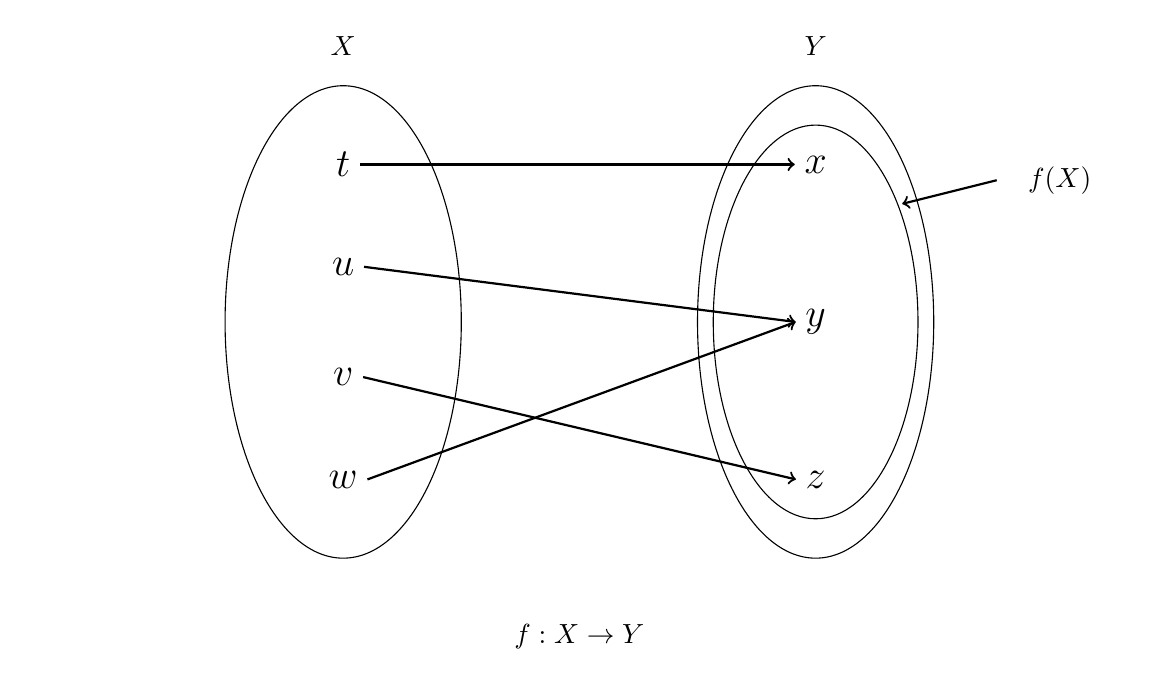
\begin{tikzpicture}
			\filldraw[white] (-7,-3) rectangle (7,3);

			\draw (-3,0) ellipse (1.5 and 3) node[yshift=3.5cm] {$X$};

			\draw (3,0) ellipse (1.5 and 3) node[yshift=3.5cm] {$Y$};
			\draw (3,0) ellipse (1.3 and 2.5);
			\draw[thick, ->] (5.3,1.8) node[xshift=.8cm] {$f(X)$} -- (4.1,1.5);

			\node (t) at (-3,2) {\Large$t$};
			\node (u) at (-3,.7) {\Large$u$};
			\node (v) at (-3,-.7) {\Large$v$};
			\node (w) at (-3,-2) {\Large$w$};

			\node (x) at (3,2) {\Large$x$};
			\node (y) at (3,0) {\Large$y$};
			\node (z) at (3,-2) {\Large$z$};

			\draw[thick,->] (t.east) -- (x.west);
			\draw[thick,->] (u.east) -- (y.west);
			\draw[thick,->] (v.east) -- (z.west);
			\draw[thick,->] (w.east) -- (y.west);

			\draw (0,-4) node {$f:X\to Y$};
	\end{tikzpicture}}
	\caption{}
	\label{fig:sur}
\end{figure}

Then, when you put these together, the resulting function is a bijection as illustrated in \cref{fig:bijection}.

\begin{prop}
	Let $f:X \to Y$ be one-to-one.
	Then $f^{-1}(f(U)) = U$ for some $U \subseteq X$
\end{prop}
\begin{proof}
	Suppose $x\in f^{-1}(f(U))$, then there exists some $y\in f(U)$ such that $f(x)=y$.
	Since $y\in f(U)$, there exists some $x'\in U$ such that $f(x')=y$.
	Thus, $f(x)=f(x')$ whereby the definition of one-to-one, we have $x=x'$ implying $x \in U$; thus we obtain $f^{-1}(f(U)) \subseteq U$.

	By \cref{prop:preimgimg}, we have $U \subseteq f^{-1}(f(U))$, thus we conclude with $f^{-1}(f(U)) = U$ thereby completing the proof.
\end{proof}

\begin{prop} \label{prop:sur-img-preimg}
	Let $f:X \to Y$ be onto $Y$.
	Then $f(f^{-1}(V)) = V$ for some $V \subseteq Y$
\end{prop}
\begin{proof}
	See \cref{exer:sur-img-preimg}.
\end{proof}

\begin{prop} \label{prop:injection-fiber-single}
	A function $f:X \to Y$ is one-to-one if and only if its nonempty fibers are singletons.
\end{prop}
\begin{proof}
	For the forwards direction, suppose $f$ is one-to-one.
	For any $y\in Y$ such that $f^{-1}(y)\neq\varnothing$, choose any $x,x'\in f^{-1}(y)$, then we have $f(x)=f(x')=y$.
	Since $f$ is one-to-one, $x=x'$; thus $f^{-1}(y)$ is a singleton.

	For the backwards direction, suppose all non-empty fibers of $f$ are nonempty.
	Then suppose $f(x)=f(x')$.
	By definition $f^{-1}(f(x))$ is nonempty and contains $x$ and $x'$.
	Since nonempty fibers are singletons, we require $x=x'$ thus proving $f$ is one-to-one.
\end{proof}

\begin{prop} \label{prop:sur-full-image}
	A function $f: \to Y$ is onto $Y$ if and only if the range of $f$ is $Y$.
\end{prop}
\begin{proof}
	Immediate by comparing the definition of range and an onto function.
\end{proof}


\begin{figure}
\centering
\resizebox{0.7\linewidth}{!}{
	\begin{tikzpicture}
		\filldraw[white] (-7,-3) rectangle (7,3);

		\draw (-3,0) ellipse (1.5 and 3) node[yshift=3.5cm] {$X$};

		\draw (3,0) ellipse (1.5 and 3) node[yshift=3.5cm] {$Y$};
		\draw (3,0) ellipse (1.3 and 2.5);
		\draw[thick, ->] (5.3,1.8) node[xshift=.8cm] {$f(X)$} -- (4.1,1.5);

		\node (u) at (-3,2) {\Large$u$};
		\node (v) at (-3,0) {\Large$v$};
		\node (w) at (-3,-2) {\Large$w$};

		\node (x) at (3,2) {\Large$x$};
		\node (y) at (3,0) {\Large$y$};
		\node (z) at (3,-2) {\Large$z$};

		\draw[thick,->] (u.east) -- (y.west);
		\draw[thick,->] (v.east) -- (z.west);
		\draw[thick,->] (w.east) -- (x.west);

		\draw (0,-4) node {$f:X\to Y$};
	\end{tikzpicture}}
	\caption{}
	\label{fig:bijection}
\end{figure}

\begin{prop} \label{prop:comp-in-sur-bi}
	Let $f:X \to Y$ and $g: Y \to Z$ be functions, then the following hold:
	\begin{enumerate}
		\item If $f$ and $g$ are one-to-one, then $g\circ f$ is one-to-one,
		\item if $f$ and $g$ are onto, then $g\circ f$ is onto,
		\item if $f$ and $g$ are bijective, then $f\circ g$ is bijective.
	\end{enumerate}
\end{prop}
\begin{proof}
	See \cref{exer:comp-in-sur-bi}.
\end{proof}

With this newfound vocabulary, we are one step closer to talking about inverses, but before we do, we must discuss function composition.
When we compose functions, we take the output from one function and put it into another.
Because of some properties of this operation resemble multiplication, the symbol we often use for composition often looks like multiplication.\footnote{
	If you ever take linear algebra, function composition distributes on addition very similarly to how multiplication does.
	It also has an interesting connection to matrix multiplication, which could be a source of motivation for the symbol.}

\begin{define}
	Define $f:Y\to Z$ and $g:X\to Y$. The composition of $f$ and $g$, notated as $f\circ g$ is a function $f\circ g:X\to Z$ such that $(f\circ g)(x)=f(g(x))$.
\end{define}

An important property that's useful later is that functional composition is associative, or $f\circ (g\circ h)=(f\circ g) \circ h$. The proof is straightforward, thus left for the reader.
Composition is also illustrated in \cref{fig:comp}.

\begin{figure}
\centering
\resizebox{0.8\linewidth}{!}{
	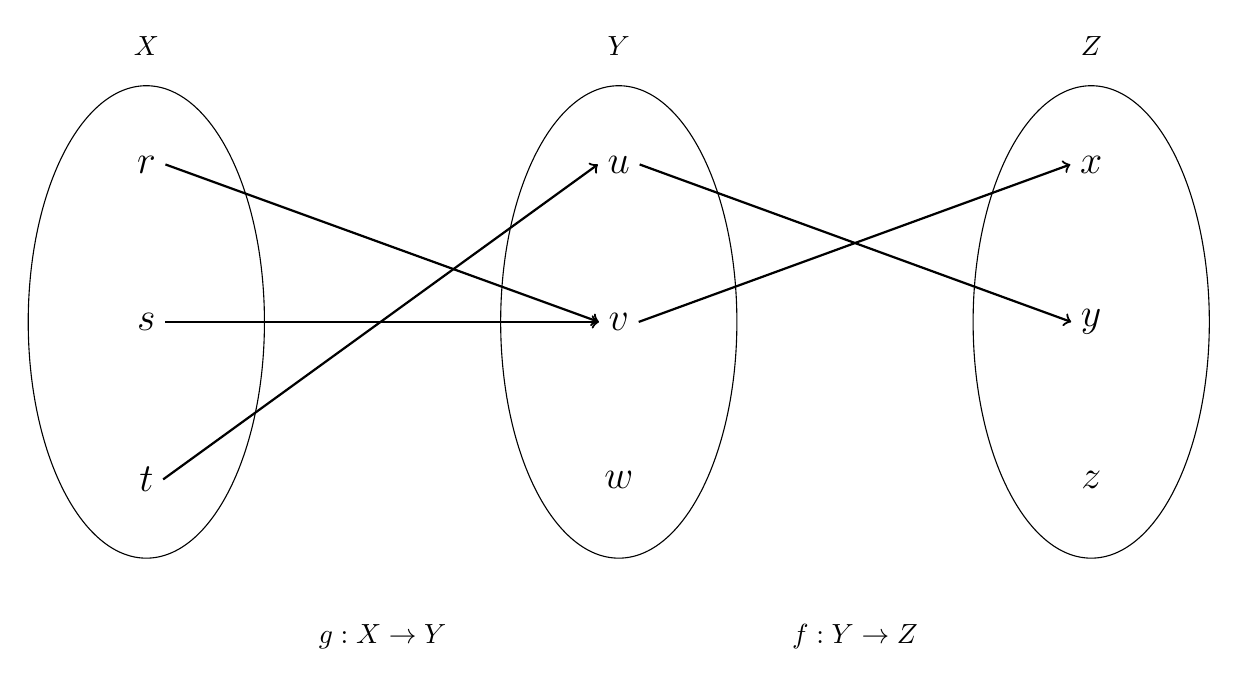
\begin{tikzpicture}
		\draw (-3,0) ellipse (1.5 and 3) node[yshift=3.5cm] {$X$};

		\draw (3,0) ellipse (1.5 and 3) node[yshift=3.5cm] {$Y$};

		\draw (9,0) ellipse (1.5 and 3) node[yshift=3.5cm] {$Z$};

		\node (r) at (-3,2) {\Large$r$};
		\node (s) at (-3,0) {\Large$s$};
		\node (t) at (-3,-2) {\Large$t$};

		\node (u) at (3,2) {\Large$u$};
		\node (v) at (3,0) {\Large$v$};
		\node (w) at (3,-2) {\Large$w$};

		\node (x) at (9,2) {\Large$x$};
		\node (y) at (9,0) {\Large$y$};
		\node (z) at (9,-2) {\Large$z$};

		\draw[thick,->] (r.east) -- (v.west);
		\draw[thick,->] (s.east) -- (v.west);
		\draw[thick,->] (t.east) -- (u.west);

		\draw[thick,->] (u.east) -- (y.west);
		\draw[thick,->] (v.east) -- (x.west);

		\draw (0,-4) node {$g:X\to Y$};
		\draw (6,-4) node {$f:Y\to Z$};
	\end{tikzpicture}}
	\caption{}
	\label{fig:comp}
\end{figure}

\begin{define} \label{def:left}
	Let $f:X\to Y$ be a function. If $g: Y\to X$ is a function such that $g\circ f=\id_X$, then $g$ is the retraction (left inverse) of $f$.
\end{define}

We take $\id_X$ in definition \eqref{def:left} as the following:

\begin{define}
	For any set $X$, let $\id_X:X \to X$ denote the \textit{identity} function on $X$ defined by $\id_X(x)=x$, for any element $x \in X$.\footnotemark
\end{define}
\footnotetext{Notice any composition with the identity function results in the same function (e.g., $f\circ \id_X=\id_Y\circ f=f$).}

\begin{define}
	Let $f:X\to Y$ be a function. If $g: Y\to X$ is a function such that $f\circ g=\id_Y$, then $g$ is the section (right inverse) of $f$.
\end{define}

An example of a retraction is illustrated in \cref{fig:left}.
Likewise, an example of a section is illustrated in \cref{fig:right}.

\begin{figure}
\centering
\resizebox{0.8\linewidth}{!}{
	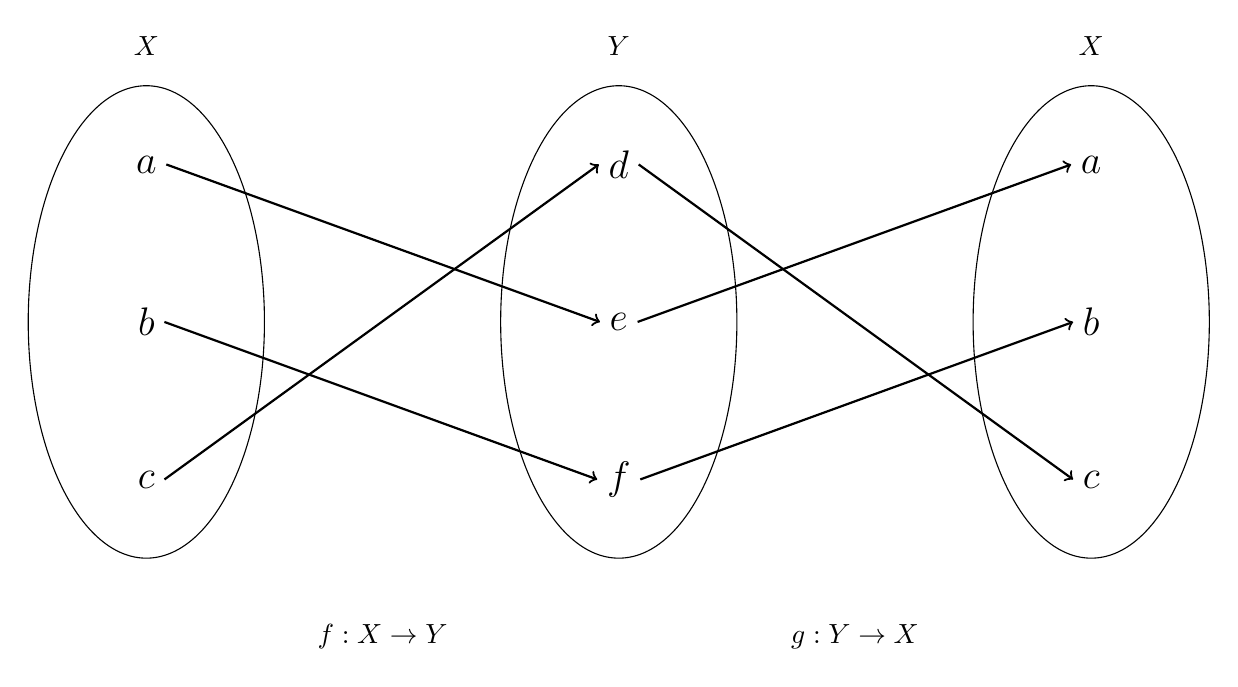
\begin{tikzpicture}
		\draw (-3,0) ellipse (1.5 and 3) node[yshift=3.5cm] {$X$};

		\draw (3,0) ellipse (1.5 and 3) node[yshift=3.5cm] {$Y$};

		\draw (9,0) ellipse (1.5 and 3) node[yshift=3.5cm] {$X$};

		\node (a) at (-3,2) {\Large$a$};
		\node (b) at (-3,0) {\Large$b$};
		\node (c) at (-3,-2) {\Large$c$};

		\node (d) at (3,2) {\Large$d$};
		\node (e) at (3,0) {\Large$e$};
		\node (f) at (3,-2) {\Large$f$};

		\node (g) at (9,2) {\Large$a$};
		\node (h) at (9,0) {\Large$b$};
		\node (i) at (9,-2) {\Large$c$};

		\draw[thick,->] (a.east) -- (e.west);
		\draw[thick,->] (b.east) -- (f.west);
		\draw[thick,->] (c.east) -- (d.west);

		\draw[thick,->] (e.east) -- (g.west);
		\draw[thick,->] (f.east) -- (h.west);
		\draw[thick,->] (d.east) -- (i.west);

		\draw (0,-4) node {$f:X\to Y$};
		\draw (6,-4) node {$g:Y\to X$};
	\end{tikzpicture}}
	\caption{}
	\label{fig:left}
\end{figure}

\begin{figure}
\centering
\resizebox{0.8\linewidth}{!}{
	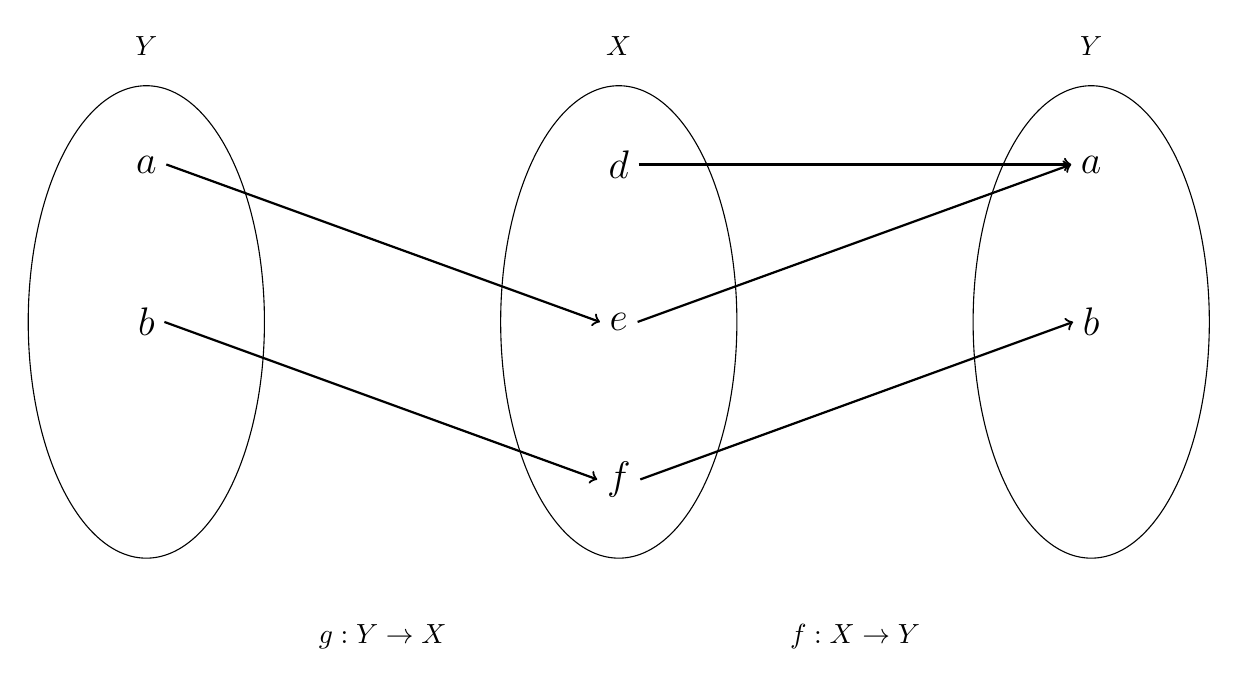
\begin{tikzpicture}
		\draw (-3,0) ellipse (1.5 and 3) node[yshift=3.5cm] {$Y$};

		\draw (3,0) ellipse (1.5 and 3) node[yshift=3.5cm] {$X$};

		\draw (9,0) ellipse (1.5 and 3) node[yshift=3.5cm] {$Y$};

		\node (a) at (-3,2) {\Large$a$};
		\node (b) at (-3,0) {\Large$b$};

		\node (d) at (3,2) {\Large$d$};
		\node (e) at (3,0) {\Large$e$};
		\node (f) at (3,-2) {\Large$f$};

		\node (g) at (9,2) {\Large$a$};
		\node (h) at (9,0) {\Large$b$};

		\draw[thick,->] (a.east) -- (e.west);
		\draw[thick,->] (b.east) -- (f.west);


		\draw[thick,->] (e.east) -- (g.west);
		\draw[thick,->] (f.east) -- (h.west);
		\draw[thick,->] (d.east) -- (g.west);

		\draw (0,-4) node {$g:Y\to X$};
		\draw (6,-4) node {$f:X\to Y$};
	\end{tikzpicture}}
	\caption{}
	\label{fig:right}
\end{figure}

To understand these concepts more, let's prove some basic properties of these inverse.

\begin{theorem} \label{thm:left}
	$f:X \to Y$ is one-to-one with $X\neq\varnothing$ if an only if $f$ has a retraction.
\end{theorem}
\begin{proof}
	For the forward direction, suppose $f$ is one-to-one and $X \neq \varnothing$.
	We have some $x_0 \in X$ since $X$ is nonempty and nonempty fibers are singletons by \cref{prop:injection-fiber-single}.
	Then construct $g: Y \to X$ by
	\begin{equation}
		g(y):=
		\begin{cases}
			f^{-1}(y)	\quad &\text{if } f^{-1}(y) \neq \varnothing \\
			x_0, 		\quad &\text{if} f^{-1}(y) = \varnothing
		\end{cases}\footnotemark
	\end{equation}
	and one can check $g$ indeed satisfies the criteria to be a function as specified in \cref{def:function}.
	By computation, we have
	\begin{equation}
		(g\circ f)(x)=g(f(x))=x
	\end{equation}
	thus $g$ is indeed the retraction of $f$ as required.
	\footnotetext{Small abuse of notation here: $f^{-1}(y)$ refers to the element contained in the one-point-set.}

	For any $x_1 x_2\in X$ such that $f(x_1)=f(x_2)$, let $g:Y\to X$ be the left inverse of $f$. Therefore, by the definition of the function, we have
	\begin{equation}
		g(f(x_1))=g(f(x_2)).
	\end{equation}
	But since $g\circ f=I_x$, we deduce $x_1=x_2$
	hence $f$ is one-to-one.
\end{proof}

\begin{theorem} \label{thm:right}
The function $f:X \to Y$ is surjective if and only if $f$ has a section.\footnotemark
\end{theorem}
\begin{proof}
	For the forward direction see \cref{prop:aoc-sections}.
	%TODO: add prop

	For the backwards direction, suppose $f$ has a section $g$. Then $f \circ g = id_Y$.
	We have
	\begin{equation}
		f(g(Y))=\id_Y(Y)=Y.
	\end{equation}
	Since $g(Y) \subseteq X$, $f(g(Y) \subseteq f(X)$, we have $Y \subseteq f(X)$.
	Therefore, $f(X)=Y$, since $f(X) \subseteq Y$ by definition.
	By \cref{prop:sur-full-image}, $f$ is surjective.
\end{proof}
\footnotetext{
	Note we don't need the nonempty criteria on $X$ since if $X$ is empty, $f$ can't be surjective. See \cref{exer:empty-surjection}
}

\begin{define}
	Let $f:X \to Y$ be a function. Then $f^{-1}:Y \to X$ is the \textit{two-sided inverse} of $f$ if and only if $f \circ f^{-1} = \id_Y$ and $f^{-1}\circ f = \id_X$.
\end{define}

Form here on out, the word \textit{inverse} is defined to mean the \textit{two-sided inverse} unless otherwise specified.

\begin{theorem} \label{thm:bi}
	A function $f:X \to Y$ has an inverse if and only if $f:X \to Y$ is a bijection.
\end{theorem}
\begin{proof}
	The forward direction is immediate by \cref{thm:left} and \cref{thm:right}, since the inverse is also the retraction and section of $f$.

	The existence the inverse on each side is given by \cref{thm:left} and \cref{thm:right}.
	Then \cref{exer:bi-unique} shows these functions are the same, thus completing the proof.
\end{proof}

Working with one-to-one, onto, or bijective functions can be incredibly useful in math, but functions in general can't be characterized by any of these adjectives.
Thus, let's introduce some function operations to facilitate with this.

\begin{define}
	Let $f:X\to Y$. Then we define $f| _A: A\to Y$, where
	$f|_A(a):=f(a)$, to be the \textbf{restriction of $f$ on $A$}
\end{define}
\begin{define}
	Let $f:X\to Y$. Then if $f|^B:X\to B$, where $f|^B(x):=f(x)$, is a well-defined function, then we call $f|^B$ the \textbf{corestriction of $f$ on $B$}.
\end{define}

We note that whilst the restriction of a function always exists, so long as $A$ is non-empty, the corestriction might not always be a well-defined function.
So, let's examine what guarantees the existence of $f|^B$.

\begin{prop}
	Suppose $f:X\to Y$.
	$f|^B$ is a function if and only if $f(X)\subseteq B$.
	\label{prop:well-def-core}
\end{prop}
\begin{proof}
	Suppose $f|^B$ is a function and let $y\in f(X)$.
	Then, by the definition of an image, there exists $x\in X$ such that $f(x)=y$. Then, by the definition of $f|^B$,
	$$f(x)=f|^B=y.$$
	Since $f|^B$ is a function, we have $y\in B$ implying $f(X)\subseteq B$.

	Then suppose $f(X)\subseteq B$. Then, we prove $f|^B$ is a function by checking with \cref{def:function}.
	First, we check that $f|^B$ satisfies (1). This is done by noticing that for every $x\in X$, we have
	$$f|^B(x)=f(x)\in f(X)\subseteq B,$$
	hence $f|^B$ satisfies (1).

	To show $f|^B$ satisfies (2), we notice if $x_1,x_1\in X$$x_1=x_2$, we have
	$$f|^B(x_1):=f(x_1)=f|^B(x_2):=f(x_2).$$
	Since $f$ is a well-defined function, we have $x_1=x_2$.
\end{proof}

By observing the definition of the corestriction and condition that a function is onto, we have the following theorem:

\begin{prop} \label{prop:co-onto}
	For any $f:X\to Y$, if $B\supseteq f(X)$, then $f|^B$ is a onto $B$.
\end{prop}
\begin{proof}
	Let $B=f(X)$. By \cref{prop:well-def-core}, $f$ satyfies the condition to be a function.
	Observe \cref{prop:sur-full-image}, $f$ is clearly onto $B$.
\end{proof}

The proposition makes the following result immediate:

\begin{cor}
	Let $f:X \to Y$ be one-to-one, then $f$ corestricts to a bijection.
\end{cor}

Similarly, we can always restrict a function to be one-to-one.

\begin{prop} \label{prop:re-one}
	For any $f:X\to Y$, there exists $f|_A$, $A\subseteq X$	where $f|_A$ is one-to-one.
\end{prop}
\begin{proof}
	By \cref{prop:co-onto}, we have $f(X)$ such that $f|^{f(X)}$ such that the corestriction is surjective.
	Thus $f|^{f(X)}$ admits a section $g:f(X) \to X$ such that $f|^{f(X)} \circ g = \id_{f(X)}$ by \cref{thm:right}.
	Take $A:=g(f(X))$, we show this makes $f$ one-to-one.

	Suppose for $x_1, x_2\in A$, suppose $f(x_1)=f(x_2)$.
	By definition, $x_1=g(y_1)$ and $x_2=g(y_2)$ for some $y_1,y_2 \in f(X)$.
	Since we have
	\begin{align}
		&f(x_1)=f|^{f(X)}(x_1)=f|^{f(X)}(g(y_1))=\id_Y(y_1)=y_1 \\
		&f(x_2)=f|^{f(X)}(x_2)=f|^{f(X)}(g(y_2))=\id_Y(y_2)=y_2
	\end{align}
	Therefore, by $f(x_1)=f(x_2)$, we have $y_1=y_2$.
	Since $g$ is well-defined, we  require $x_1=x_2$ thus proving proposition.
\end{proof}

Since sections need not be unique for a function, the restriction here is not unique,
In general, for an arbitrary function the restriction down to an injection may not be of much use, but in cases where we have chosen a particular section, this theorem provides an algorithm for producing an injection compatible with the given section.
We should also note the restriction here promotes any section to a two-sided inverse as the corestriction of the restriction on its image gives a bijection.
It follows that the section is the unique inverse on the resulting function.

%TODO: Add examples of inverses and things.

\begin{prop} \label{prop:prod-func-eq}
	For any set $X$, there exists a bijection of the form $\prod_{x \in X} Y \to Y^X$.
\end{prop}
\begin{proof}
	Define $\phi: \prod_{x \in X} Y \to Y^X$ such that $\phi((c_i)_{i\in X})(x)=c_x$.
	One can easily check that this is a well-defined function.

	Then suppose $\phi((c_x)_{x\in X})(x)=\phi((c_x)_{x \in X})(x)$.
	The function definition implies for each $x\in X$, $c_x = c'_x$.
	Therefore $(c_x)_{x \in X} = (c_x')_{x \in X}$ implying $\phi$ is injective.

	For surjectivity, for each $f(x) \in Y^X$, construct the tuple $(f(x))_{x \in X}$.
	Then by definition, this tuple maps to $f$ under $\phi$.
	Therefore, $\phi$ is the bijection as desired.
\end{proof}

We can extend \cref{prop:prod-func-eq} to arbitrary products by replacing $Y^X$ with the subset
\begin{equation}
	\{f \in C^I \mid f(i) \in C_I\}
\end{equation}
where $C$ is the union of the collection $\mathcal C$ and $I$ is an indexing on $\mathcal C$ (see exercise \cref{exer:prod-func-eq}).

If back to the definition of a bijection, we can think of them as pairings of elements between two sets.
For this reason, we can think of a bijection as simply a relabeling map which identifies every object in a set with a new representation in another set and vise versa.
Think of bijections in this way, what \cref{prop:prod-func-eq} tells us is that the set of functions and the set of tuples are the same set up to some relabeling.
This idea of objects being the same up to some relabeling is very common and we often denote these relations as \textit{isomorphisms}.\footnote{We often reserve the term \textit{isomorphism} to situations where there is something other than the set structure being preserved. We will touch on this later when we construct more complicated mathematical objects.}

For two sets under bijection, while these two sets may not be equivalent as sets (i.e. they don't contain precisly the same elements), since the specific interpretation of each element in a set doesn't really matter for most applications (and for much of math for that matter), bijective equivilence is as strong of an conclusion as one will ever need in set theory.\footnote{For a set with nothing else defined, generally, the only property that we are interested in preserving is the \textit{number of elements} a set contains, which bijections do a perfectly fine job of preserving.}
For example, the set of natural numbers, whilst traditionally represented by Arabic numerals, would functionally still be the natural numbers even if we replaced every symbol with random Egyptian hieroglyphics, just so long as the interactions between the symbols are retained to some degree (like the ordering properties, or the way two symbols add or multiply).
As we get further in math, we find that we generally stop giving individual symbols in set specific interpretations and only provide a definition of how these symbols interact.

\section{Cardinality}
A natural property that sets have is their \textit{cardinality} or in other words, the number of elements in a set.
For the finite case, this is a rather simple as a finite algorithm always exist\footnote{One can always in theory just count the number of elements of any arbitrary large finite set. Since the sets in question are finite, the algorithm will always be completed in finite time (albeit sometimes the entire will take longer than the age of the universe.)} which compares the sizes of any two sets.
However, this primitive method of comparing sets would not work in the infinite case.
Thus, if we restrict ourselves to this rather primitive method of comparing cardinality, we severely limit our understanding of sets.
To study infinite sets, set theory provides us a very useful generalization of our intuitive notion of size so that we can better understand sets that extend beyond infinity.

For this section, to save some on some clutter, I will leave the proofs of various injections, surjections, and bijections that I've determined to be rather elementary as exercises for the reader, for I find many of these proofs are unimportant to the main arguments presented in this section.

\begin{define} \label{def:cardinality}
	Let $X$ and $Y$ be sets.
	$X$ and $Y$ has the same cardinality if and only if there exists a bijection $f:X \to Y$.
\end{define}

When two sets $X$ and $Y$ have the same cardinality, we often denote this relation by $|X|=|Y|$.
As suggested by the choice of notation, this is indeed an equivalence relation (see \cref{exer:card-eq}).\footnote{
	If were to be a bit picky, our definition of a relation works between two sets.
	However, if we pause to pose the question \textit{what set does this relation operate over}, we would quickly come to the conclusion the set in question would have to be \textit{the set of all sets}.
	If were a bit more formal about our definitions of a set here, we would quickly find the \textit{set of all sets} is not in fact a set (see final section of this chapter).
	What we have here instead is not a relation between two sets but rather a relation between two \textit{proper classes}, or collection of objects that don't form a set.
	In particular, our relation relates objects between the \textit{class of all sets}.
}
This intuitive formalizes the idea of comparing two sets by writing two sets in a side-by-side table.
The two lists are identical if and only if there is a bijection between the two sets.

We can also define an order relation on set cardinality by the following:
\begin{define}
	$X$ and $Y$ are sets such that $|X|\le |Y|$ if and only if there is an inclusion $X \to Y$.
\end{define}

One should check that this indeed forms a linear ordering  on equivalence classes of sets with equal cardinality (see \cref{exer:card-order}).
In particular \cref{prop:card-well-order} shows this ordering satisfies the conditions to be a well-ordering.
In search of a solution, one might make use of the following result:
%TODO: add this proposition

\begin{lemma}
	Let $X$ and $Y$ be sets. Suppose there exists the inclusion $f:X \to Y$ and surjection $g:X \to Y$.
	Then there exists a bijection $X \to Y$.
\end{lemma}
\begin{proof}
	%TODO: Finish This
\end{proof}

Let us also note the following useful results.

\begin{prop} \label{prop:subset-card}
	Suppose $W \subseteq X$, then $|W| \le |X|$.
\end{prop}
\begin{proof}
	The restriction $\id \mid _W$ (also known as the canonical injection) is injective thus providing the conclusion.
\end{proof}

\begin{prop} \label{prop:set-neq-power}
	For any set $X$, $X < |P(X)|$.
\end{prop}
\begin{proof}
	Let $i:X \to |P(X)|$ be the function such that $i(x):= \{x\}$.
	Clearly, $\phi$ is injection thus $X < |P(X)|$.

	Then notice, for the subset
	\begin{equation}
		W := \{x \in X \mid x \notin \phi(x)\},
	\end{equation}
	for any $x\in X$ such that $x \in W$, $\phi(x) \neq W$ since $x \notin \phi(x)$.
	Conversely for any $x\in X$ such that $x \notin W$, $\phi(x) \neq W$ since $x\in \phi(x)$.
	Therefore, $W$ is not in the range of $\phi$.
	This shows a bijection between $X$ and $P(X)$ cannot exist thus $|X|\neq|P(X)|$ thereby proving the proposition.
\end{proof}

\subsection{Finite Sets}
To explore this concept more, let's first talk about the simplicist type of sets: Finite sets.
Let's begin by giving a formal definition of what we're about to discuss.

\begin{define}
	A $X$ is finite if $|X|=|N_n|$, for some $n\ge 0$, where
	$$N_n := \{m\in \nat \mid m \le n\}.$$
\end{define}

One can check this indeed formalizes the intuitive understanding of a finite set.
Let's make a few observations.

\begin{prop} \label{prop:finite-in-sur-bi-eq}
	For finite sets $X$ and $Y$ such that $|X|=|Y|$, the following are equivalent:
	\begin{enumerate}
		\item $f:X\to Y$ is one-to-one,
		\item $f:X \to Y$ is onto $Y$,
		\item $f:X \to Y$ is a bijection.
	\end{enumerate}
\end{prop}
\begin{proof}
	Given 3, 1 and 2 follows trivially.

	We prove $1 \implies 3$
	Suppose $f:X \to Y$ is one-to-one.
	Since $X$ and $Y$ are finite, we have for some $n$
	\begin{equation}
		|X|=|Y|=|N_n|
	\end{equation}
	We proceed by induction on $n$.
	\Cref{exer:zero-card-set} shows $\varnothing$ is unique set such that $|X|=|N_0|$.
	Thus functions between $N_0$ cardinality sets must be of the form $f:\varnothing \to \varnothing$.
	By \cref{prop:unique-empty-function}, only one such functions exists and one can check this unique function is a bijection.

	For inductive step, suppose if $f:X \to Y$ is one-to-one for $|X|=|Y|=|N_n|$, then it's onto $Y$.
	Then for $|X'|=|Y'|=|N_{n+1}|$, for any $f':X'\to Y'$ that is one-to-one, by the cardinality of $X'$, there exists $\rho:N_{n+1} \to X'$ that is a bijection.
	The restriction $f'\mid_{X' \setminus \{x_0\}}$ is one-to-one into $Y' \setminus \{y\}$ for $x_0= \rho(n+1)$ and $y_0=f'(x_0)$.
	If we show
	\begin{equation}
		|X' \setminus \{x_0\}|=|Y' \setminus \{y_0\}|=|N_n|,
	\end{equation}
	the inductive hypothesis concludes the restriction of $f'\mid_{X' \setminus \{x_0\}}$ is onto $Y' \setminus \{y_0\}$ and thus $f'$ is one-to-one onto $Y'$.

	The restriction $\rho_{N_{n+1}\smallsetminus \{n+1\}}$ is clearly one-to-one onto $X' \setminus \{\rho(n+1)\}$.
	Since $|Y|=|N_{n+1}|$, there exists bijection $\tau:N_{n+1} \to Y$.
	Define $\sigma: N_{n+1} \to N_{n+1}$ such that
	\begin{equation}
		\sigma(k) :=
		\begin{cases}
			k 				\quad &\text{if } k \neq n+1 \text{ or } \tau^{-1}(y_0), \\
			n+1 			\quad &\text{if } k=\tau^{-1}(y_0), \\
			\tau^{-1}(y_0)	\quad &\text{if } k=n+1.
		\end{cases}
	\end{equation}
	$\sigma$ is a bijection, and in particular the composition $\tau \circ \sigma$ is a bijection by \cref{prop:comp-in-sur-bi} and $(\tau\circ \sigma)(n+1)=y_0$.
	Following the same argument for the $X'$ case, $|Y' \setminus \{y_0\}|=|N_n|$.

	$2 \implies 3$ follows from $1\implies 3$ by observing every surjective function admits a section.
	The section is one-to-one, thus $1\implies 3$ implies this section is a bijection.
	Thus, it suffices by showing these facts imply original function must be a bijection (see \cref{exer:finite-sur-in}).
\end{proof}

The previous theorem has the following consequences:

\begin{cor} \label{cor:unique-nat-finite-card}
	 $m \neq n$ if and only if $|N_m| \neq |N_n|$.
\end{cor}
\begin{proof}
	Let $m \neq n$.
	Then suppose without loss of generality, $m < n$, then we have the canonical injection $i:N_m \to N_n$ since $N_m \subseteq N_n$.
	This inclusion is clearly not surjective, thus by \cref{prop:finite-in-sur-bi-eq}, we conclude $|N_m|\neq |N_n|$.

	The reverse direction is trivial.
\end{proof}

\begin{cor} \label{cor:nat-finite-card-ineq}
	$m \le n$ if and only if $|N_m| \le |N_n|$
\end{cor}
\begin{proof}
	The canonical injection $N_m \to N_n$ for $m \le n$ makes the forward direction immediate.

	For the reverse direction, suppose $m > n$, then we have the obvious inclusion $i: N_n \to N_m$, thus $|N_m| \ge |N_n|$.
	\Cref{cor:unique-nat-finite-card} implies this inequality is strict thus $|N_m| > |N_n|$.
\end{proof}

\Cref{cor:unique-nat-finite-card} makes precise the observation that sets with $m$ and $n$ elements for $m\neq n$ aren't the same size, a rather unremarkable fact given our intuitive understanding of the world.
Mathematically, it also means that the function
\begin{equation}
	\nat \cup \{0\} \to \mathcal{F}_\sim, \quad n \mapsto  |N_n|\footnotemark
\end{equation}
is bijective, for $\mathcal{F}_\sim$ is the class (since the collection of all finite sets is not itself a set for technical reasons) of equivalence classes of finite sets identified by cardinality.\footnote{
	For the set theorist out there, I'm being very imprecise with my definitions on purpose to avoid confusion.
	In particular, taking the collection of equivalence classes on a proper class requires some nuance since proper classes by definition can't belong to any class.
	We will ignore this here since it's unimportant to the argument which I construct here.
}
One should also check that this function is well-defined and surjective (see \cref{exer:finite-set-map-to-nat}).
\footnotetext{The symbol $a \mapsto b$ indicates $f(a) = b$ for a function $f:A \to B$.}
Consequently, this class function allows us to uniquely identify each finite set with a natural number corresponding to its size making precise the statement \textit{$X$ is a set of $m$ elements}.
With a bit of abuse of notation, we often denote the cardinality of a finite set $X$ of $m$ elements by $|X|=m$.
Finally, \cref{cor:nat-finite-card-ineq} says the class bijection also preserves the order relation (i.e $m \le n$ implies $|N_m| \le |N_n|$).
This makes precise the statement \textit{a set of $m$ elements is larger than a set of $n$ elements for $m \le n$}.

\begin{cor} \label{cor:finite-subset-card}
	Suppose $W \subsetneq X$, then $|W| < |X|$.
\end{cor}
\begin{proof}
	\Cref{prop:subset-card} gives use $|W| \le |X|$.
	Since the canonical inclusion $W \to X$ is not an onto, since $W$ is a proper subset, \cref{prop:finite-in-sur-bi-eq} implies $|W| \neq |X|$, thus we obtain our conclusion.
\end{proof}

\Cref{cor:finite-subset-card} makes the statement in \cref{prop:subset-card} stronger in the case of finite sets which formalizes the idea that subcollection is strictly smaller than the original collection.
This observation, however, generally doesn't hold in the case of infinite sets as we will see later.

\Cref{prop:finite-in-sur-bi-eq} also gives us the following useful result:

\begin{thm}[Pigeonhole Princciple] \label{thm:pigeonhole}
	Suppose $X$ and $Y$ are finite sets such that $|X| > |Y|$ and the function $f:X \to Y$ is onto $Y$.
	Then $f$ is not one-to-one.
\end{thm}
\begin{proof}
	See \cref{exer:pigionhole}
\end{proof}

This formalizes the observation that if we have $m$ boxes and $n$ items such that $m<n$, one box must contain more than one item.
The following examples show how this concept can be used in math.

%TODO: add pigion hole examples.

\begin{prop} \label{prop:card-arith}
	Suppose $|X|=m$ and $|Y|=n$, then the following hold:
	\begin{enumerate}
		\item $|X \cup Y| = m + n$ for $X\cap Y=\varnothing$,
		\item $|X \times Y| = mn$,
		\item $|X \setminus W|$ for $W \subseteq X$.
	\end{enumerate}
\end{prop}
\begin{proof}
	This proposition is proved by explicitly constructing the required bijections (see \cref{exer:card-arith}).
	%TODO: add exercise.
\end{proof}

\begin{thm} (Inclusion-Exclusion Principle)
	Suppose $X$ and $Y$ are finite sets, then
	\begin{equation}
		|X\cup Y| = |X| + |Y| - |X \cap Y|
	\end{equation}
\end{thm}
\begin{proof}
	We have the following set identity:
	\begin{equation}
		X \cup Y = (X \setminus (X\cap Y)) \cup (Y \setminus (X\cap Y)) \cup (X \cap Y) \quad \text{see \cref{exer:ex-in-set-id}}.
	\end{equation}
	The sets $X \setminus (X\cap Y)$, $Y \setminus (X\cap Y),$ and $X \cap Y$ sets pairwise disjoint (i.e. intersection of each pair is $\varnothing$.)
	Therefore, by \cref{prop:card-arith}, we have
	\begin{align}
		|X \cup Y| &= |(X \setminus (X\cap Y)) \cup (Y \setminus (X\cap Y)) \cup (X \cap Y)| \\
			&= |X \setminus (X \cap Y)| + |Y \setminus (X \cap Y)| + |X \cap Y| \\
			&= |X| - |X \cap Y| + |Y| - |X \cap Y| + |X \cap Y|\\
			&= |X| + |Y| - |X \cap Y|
	\end{align}
\end{proof}

\begin{prop}
	If $|X|=m$ and $|Y|=n$, then $|Y^X|=n^m$
\end{prop}
\begin{proof}
	By \cref{prop:prod-func-eq} we have $|Y^X|=|\prod_{x\in X}Y|=|Y^m|$
	\Cref{prop:card-arith} gives us $|Y^m|=|Y|^m = n^m$, thereby completing the proof.
\end{proof}

These relations give us a way to compute the sizes of various finite sets.
The full study of counting sizes of finite sets will be covered in \cref{ch:combinatorics}, but here are a few basic examples using these formulae.

%TODO: Add chapter ref and add examples of combinatorics.

\subsection{Infinite Sets}
Previously, the various propositions that we proved are, so we can check that our formalism matches what our intuition tells about.
However, as we move to infinite sets, our intuition starts to breakdown and the real power of this formalism start to show.

Let's start with the following definition

\begin{define} \label{def:countable}
	A set is \textit{countable} if and only if $|X|\le|\nat|$.
	If a set is countable yet not finite, we denote these sets as \textit{countably infinite}.
\end{define}

\begin{ex} \label{ex:countable-set}
	\Cref{def:countable} tells us immediately that the set $\nat$ is countable.
	In additional, for any finite set, since there exists the canonical inclusion $N_n \to \nat$, we get that finite sets are all countable.
	In particular since for any map $f:N_n \to \nat$, the natural number
	\begin{equation}
		m:=\sum_{k \in N_n} f(i)
	\end{equation}
	is not in the range of $f$ thus $f$ is never a bijection.
	This shows $\nat$ is not finite, implying $\nat$ is countably infinite.

	We can show the following sets are also countably infinite by constructing a suitable bijection.
	To start, for any finite set $|X|=n$ (suppose without loss of generality $X \cap \nat = \varnothing$), let $\rho: N_n \to X$ be a bijection, then define
	\begin{equation}
		\phi: \nat \to \nat \cup X, \quad \phi(k):=
			\begin{cases}
				\rho(n)		\quad &\text{if } k \le n, \\
				k-n j		\quad &\text{if } k > n.\\
			\end{cases}
	\end{equation}
	$\phi$ is a bijection thus the set $\nat \cup X$ is countable.
	We can of course replace $\nat$ with any countable set, with the finite case handled in \cref{prop:card-arith} and the bijection for the infinite case can be obtained similarly by composing the $k>n$ case with the bijection $\nat \to Y$, for some arbitrary countable infinite set $Y$.

	We can also show $\integ$ is countable by considering the bijection
	\begin{equation}
		\psi:  \integ \to \nat \cup \{0\}, \quad \psi(k):=
		\begin{cases}
			2k,		\quad &\text{if } k\ge 0, \\
			-(2k+1)	\quad &\text{if } k < 0.
		\end{cases}
	\end{equation}
	Then denote the set of even integers by $2\integ$, then by the bijection,
	\begin{equation}
		\tau: \integ \to 2\integ, \quad \tau(k) = 2k
	\end{equation}
	the set of even integers is also countable.
	Since $2\integ \subseteq \integ$, this provides us for a counterexample for the claim that $W \subsetneq X$ implies $|W| < |X|$ in the case of infinite sets.
\end{ex}

\begin{prop} \label{prop:countable-product}
	Let $X$ and $Y$ be countable sets.
	Then $X\times Y$ is countable.
\end{prop}
\begin{proof}
	Let's prove the proposition for the case $\nat \times \nat$.
	By the following diagram
	\[\begin{tikzcd}
		& 1 & 2 & 3 & 4 & 5 & 6 & \dots \\
		1 & \bullet & \bullet & \bullet & \bullet & \bullet & \bullet \\
		2 & \bullet & \bullet & \bullet & \bullet & \bullet \\
		3 & \bullet & \bullet & \bullet & \bullet \\
		4 & \bullet & \bullet & \bullet \\
		5 & \bullet & \bullet \\
		6 & \bullet \\
		\vdots
		\arrow[from=2-2, to=2-3]
		\arrow[from=2-3, to=3-2]
		\arrow[from=2-4, to=2-5]
		\arrow[from=2-5, to=3-4]
		\arrow[from=2-6, to=2-7]
		\arrow[from=2-7, to=3-6]
		\arrow[from=3-2, to=4-2]
		\arrow[from=3-3, to=2-4]
		\arrow[from=3-4, to=4-3]
		\arrow[from=3-5, to=2-6]
		\arrow[from=3-6, to=4-5]
		\arrow[from=4-2, to=3-3]
		\arrow[from=4-3, to=5-2]
		\arrow[from=4-4, to=3-5]
		\arrow[from=4-5, to=5-4]
		\arrow[from=5-2, to=6-2]
		\arrow[from=5-3, to=4-4]
		\arrow[from=5-4, to=6-3]
		\arrow[from=6-2, to=5-3]
		\arrow[from=6-3, to=7-2]
	\end{tikzcd}\]
	where the first component is listed in the first column and the second component listed as the first row, following the arrows, we obtain a bijection between $\nat \times \nat \to \nat$.

	Then to prove the case where both sets are countably infinite, let $\i_X \to \nat$ and $\i_Y: Y \to \nat$ be injections.
	The function defined by
	\begin{equation}
		\phi: X \times Y \to \nat \times \nat, \quad \phi(x,y):= (i_X(y), i_Y(y)))
	\end{equation}
	is an injection.
	Therefore, $|X\times Y| \le |\nat \times \nat|=|\nat|$
\end{proof}

\begin{cor}
	Let $\mathcal{U}$ be a countable collection of countable sets.
	Then union of all sets in $U$, dented $\bigcup_{U \in \mathcal{U}} U$, is countable.
\end{cor}
\begin{proof}
	Let $i_U: U \to \nat$ be injections for each $U \in \mathcal{U}$.
	Then by \cref{thm:left}, there exist retractions $r_U: \nat \to U$ for each $U$.
	\Cref{thm:right} concludes these retractions are surjective.
	Then the function
	\begin{equation}
		\phi: \mathcal{U} \times \nat \to \bigcup_{U \in \mathcal U}, \quad  \phi(U,k):=r_U(k).
	\end{equation}
	In particular, $\phi$ is onto and thus admits a section by \cref{thm:right}.
	This section is of the form $\bigcup_{U \in \mathcal U} \to \mathcal U \times \nat$ and is injective \cref{thm:left}.
	Therefore, $|\bigcup_{U \in \mathcal U} U | \le |\mathcal U \times \nat| \le |\nat|$ by \cref{prop:countable-product}
	Thus $\bigcup_{U \in \mathcal U} U$ is countable.
\end{proof}

\begin{ex}
	\Cref{prop:countable-product} implies $\integ \times \integ$ is countable.
	Observe, since $\rat$ is the set of all reduced fractions, we can instead rewrite each fraction as an ordered pair and we observe $\rat \subseteq \integ \times \integ$.
	Since $\integ \times \integ$ is countable and canonical inclusions implies $|\rat| \le |\integ \times \integ|$, we see $\rat$ is in fact countable.

	At this point, we might conclude that every infinite set is countable, but of course this is not the case (or else there wouldn't be a dedicated chapter talking about them).
	Let's examine the set $\real$.
	We know from experience each real number can be given a decimal expansion.
	In particular, let's restrict ourselves to the interval $0\le x < 1$.
	We can view each decimal expansion as a sequence of integers ranging from 0 to 9.
	Let's denote the set of sequences of digits as $10^\nat$.
	We note since $10^\nat$ can be viewed as a subset of $\real$, we have $|10^\nat| \le \real$
	If $2^\nat$ denotes sequences of binary digits (sequences of 0 and 1), the map
	\begin{equation}
		\pi: 10^\nat \to 2^\nat, \quad \pi(d_i):=
		\begin{cases}
			1	\quad &\text{if } d_i \neq 0, \\
			0	\quad &\text{if } d_i =0
		\end{cases}
	\end{equation}
	is surjective, thus $|2^\nat|\le|10^\nat|$ by the existence of a section.
	Since the map
	\begin{equation}
		\phi:P(\nat) \to 2^\nat, \quad \phi(S)_i:=
		\begin{cases}
			0	\quad&\text{if } i\notin S \\
			1	\quad&\text{if } i\in S \\
		\end{cases}
	\end{equation}
	is a bijection,\footnote{
		We can form this bijection with any set.
		For this reason, we sometimes denote $|P(X)|=2^X$.
	} and by \cref{prop:set-neq-power}, we have
	\begin{equation}
		\nat < |P(\nat)| \le |2^\nat| \le |10^\nat|\le|\real|.
	\end{equation}
	This implies the set $\real$ is \textit{not} countable, a remarkable result since any interval in $\real$ intersects non-trivially with $\rat$\footnote{A non-trivial result we will prove in a later section.}
	We refer to non-countable sets simply as \textit{uncountable}.
	This also shows the idea that there are different sizes of infinity, something not obvious given our understanding of infinity using out intuition.
	In fact \cref{prop:set-neq-power}, we can get even larger infinities by iteratively taking the power set of $\nat$.

	If we were a bit more particular about our choice of function $10^\nat \to 2^\nat$, we could actually obtain a bijection here, since every real number also has a unique binary representation.
	In addition, a bijection can also be constructed for $[0,1) \to \real$, a fact I will leave for the reader to ponder.
	In light of these facts, we in fact have $|\real| = 2^\nat$, where $2^\nat$ denotes the cardinality of $P(\nat)$.

	However, if there's any doubt about the previous argument, let me provide visual argument of the same fact.
	For every function from $\nat$ to $0<x<1$ and , we can represent the bijection as the following list:
	\[\begin{tikzcd}
		{\textbf{1:}} & {\textcolor{red}{.1}} & 4 & 3 & 9 & 3 & \dots \\
		{\textbf{2:}} & {.2} & {\textcolor{red}{3}} & 2 & 7 & 4 & \dots \\
		{\textbf{3:}} & {.5} & 1 & {\textcolor{red}{5}} & 2 & 3 & \dots \\
		{\textbf{4:}} & {.5} & 0 & 5 & {\textcolor{red}{1}} & 2 & \dots \\
		{\textbf{5:}} & {.4} & 6 & 6 & 0 & {\textcolor{red}{2}} & \dots \\
		\vdots & \vdots & \vdots & \vdots & \vdots & \vdots & \ddots
		\arrow[from=1-2, to=2-3]
		\arrow[from=2-3, to=3-4]
		\arrow[from=3-4, to=4-5]
		\arrow[from=4-5, to=5-6]
	\end{tikzcd}\]
	Following the arrows along the diagonal, we can generate a new sequence by incrementing each digit by 1 (and wrap 9 back to 0), we generate a new sequence which by definition is different from every sequence on the list.
	Thus, our function doesn't map to it, thus this function cannot be onto the interval $0<x<1$, therefore giving us the conclusion that $\real$ is not countable.\footnote{
		This argument here is known as \textit{Canter's diagonalization argument}.
		If we trace back our first argument, we find these arguments are morally the same.}
\end{ex}

\begin{prop}
	Every countable infinite set has a bijection with $\nat$.
\end{prop}
\begin{proof}
	Suppose $X$ is countably infinite, thus there exists a injection $i:X \to \nat$.
	Then image $i(X)\subseteq \nat$ is infinite (since the corestriction by the range is a bijection by \cref{prop:co-onto}).
	It suffices to show there exists a bijection $i(X) \to \nat$.
	For each $k\in i(X)$, define
	\begin{equation}
		U_k := \{m \in i(X) \mid k \ge m \}.
	\end{equation}
	Each $U_k$ has the greatest element $k$ thus $U_k \subseteq N_k$ implies they are finite.
	Then define $\mathcal U$ to be the collection of all these sets.
	The obvious function $\psi:i(X) \to \mathcal U$ where $\psi(k):= U_k$ is clearly onto $\mathcal U$.
	It is one-to-one since if $\psi(k)=\psi(k')$, we have $U_k=U_{k'}$.
	The greatest element of each set is $k$ and $k'$ respectively thus $k=k'$ since they are the same set.

	Thus, it suffices to show the function
	\begin{equation}
		\phi: \mathcal U \to \nat, \quad \phi(U_k):= |U_k|
	\end{equation}
	is a bijection.
	Suppose $\phi(U_k)=\phi(U_{k'})$, then $|U_k|=|U_{k'}|$.
	Since the ordering on $\nat$ is linear, $k \le k'$ or $k \ge k'$.
	Without loss of generality, we can assume the former.
	Therefore, $U_k \subseteq U_{k'}$.
	Since these are finite sets with the same cardinality, the canonical injection must be the identity by \cref{prop:finite-in-sur-bi-eq}.
	Therefore, $k=k'$ follows immediately.

	To show $\phi$ is onto $\nat$, suppose $\phi(U_k)=n$.
	We will proceed by induction on $n$.
	For $n=1$, take $k$ to be the least element of $i(X)$, since $i(X)$ is the subset of a well-ordered set.
	Then $\phi(U_k)=1$

	Then suppose $\phi(U_k)=n$.
	$i(X)$ is well-ordered thus we have the successor operation.
	Every element $k$ has a successor since if it doesn't, it implies $k$ is the greatest element, and thus $i(X)\subseteq N_k$, a contradiction of the assumption $i(X)$ is infinite.
	If $k'$ is the successor of $k$, $U_{k'}=U_{k} \cup \{k'\}$, thus $\phi(U_k)=n+1$.

	By induction $\phi$ is onto, thus a bijection.
	Therefore, the composition $\phi \circ \psi: i(X) \to \nat$ is the bijection as desired.
\end{proof}

This is a nice result and would leave many wondering whether there are sets such that $|\nat|<|X|<|2^\nat|$.
Known as the \textit{continuum hypothesis}, this problem is unfortunately undecidable given the conventional formulation of set theory.
The details of why mathematicians arrive at this fact is beyond the scope of anything covered in this book and thus will be omitted.

\optionalsection{Formal View}
To be continued ...

\section{Exercises}

\begin{exercise}
	Let $A=\{1,\beta,20\}$, $B=\{\text{two},\beta,20\},C=\{20,\text{one},\alpha\}$. Give the sets resulting from
	\begin{enumerate}[topsep=1ex]
		\item $A \cup B$
		\item $A \cap B$
		\item $C \setminus A$
		\item $A \cup (B\cap C)$
	\end{enumerate}
\end{exercise}

\begin{exercise}
	Define each of the following sets in set builder notation.%
	\begin{enumerate}
		\item The interval $-5<x<3$ or $-10<x<-3$.
		\item The set of all even numbers.
		\item The set of all positive perfect squares (excluding 0).
	\end{enumerate}
\end{exercise}

\begin{exercise}~ \label{exer:product-empty}
	\begin{enumerate}[topsep=1pt]
		\item For any $I$-indexing of $\mathcal C$ such that $\varnothing \in \mathcal C$, suppose $i \in I$, $C_i = \varnothing$, then the $\prod_{i \in I} C_i = \varnothing$.
		\item For any $\varnothing$-indexing of any collection $\mathcal C$, what is $\prod_{i \in \varnothing} C_i$?
	\end{enumerate}
\end{exercise}

\begin{exercise} \label{exer:subset-trans}
	Check that the subset relation transitive.
\end{exercise}

\begin{exercise}
	Let $q$ be any real number such that $q\neq1$. Show, for any $n\in\nat$,
	$$\sum_{k=1}^nq^k=\frac{q^{n+1}-q}{q-1}.$$
\end{exercise}

\begin{exercise}
	Prove $5^n+5<5^{n+1}$ for all $n\in\nat$.
\end{exercise}

\begin{exercise}[$\dagger$]
	For any statement, $P(n)$ for $n\in\nat$, suppose
	\begin{enumerate}
		\item $P(1)$ is true
		\item For $n\in\nat$, $P(n)$ implies $P(n+2)$
	\end{enumerate}
	Prove $P(n)$ is true for every positive odd integer.
\end{exercise}

\begin{exercise} \label{exer:imgpreimg}
	For any function $f:X \to Y$, show $f(f^{-1}(V)) \subseteq V$ for any $V \subseteq Y$.
\end{exercise}

\begin{exercise} \label{exer:comp-in-sur-bi}
	Prove \cref{prop:comp-in-sur-bi}.
\end{exercise}

\begin{exercise} \label{exer:sur-img-preimg}
	Prove \cref{prop:sur-img-preimg}.
\end{exercise}

\begin{exercise} \label{exer:preimg-imgbi}
	Suppose $f:X \to Y$ is a bijection with inverse $g: Y \to X$. Then the preimage $f^{-1}(B) = g(B)$ for any $B \subseteq Y$.
\end{exercise}

\begin{exercise} \label{exer:empty-surjection}
	Any function of the form $\varnothing \to Y$ can't be onto $Y$.
\end{exercise}

\begin{exercise}~ \label{exer:bi-unique}
	\begin{enumerate}
		\item Suppose $f:X \to Y$ is a bijection. Show $f$ has a unique inverse.
		\item Let $r:Y \to X$ and $s: Y \to X$ be the retraction and section of $f$ given by \cref{thm:left} and \cref{thm:right}.
			Show that these are necessarily the same function.
	\end{enumerate}
\end{exercise}

\begin{exercise} \label{exer:prod-func-eq}
	Let $\mathcal C$ be some collection of sets.
	Then for any $I$-indexing of $\mathcal C$, show there is a bijection of the form $\prod_{i \in I} C_i \to \{f \in C^I \mid f(i) \in C_I\}$, for $C$ is the union of the collection $\mathcal C$.
\end{exercise}

\begin{exercise} \label{exer:card-eq}
	Show that the relation $|X|=|Y|$ is an equivalence relation on the class of sets.
\end{exercise}

\begin{exercise} \label{exer:card-order}
	Check that the relation $|X| \le |Y|$ forms a linear ordering on the equivalence classes of the cardinality equivalence relation.
\end{exercise}

\begin{exercise} \label{exer:zero-card-set}
	Show $\varnothing$ is unique set with cardinality zero (has cardinality $N_0$).
\end{exercise}

\begin{exercise} \label{exer:finite-sur-in}
	Show for a finite set $X$ and $Y$, any surjection $f:X \to Y$ is a bijection following the hint in the proof of \cref{prop:finite-in-sur-bi-eq}.
\end{exercise}

\begin{exercise} \label{exer:finite-set-map-to-nat}
	Show
	\begin{equation}
		\nat \cup \{0\} \to \mathcal{F}_\sim, \quad n \mapsto  |N_n|
	\end{equation}
	is a bijection.
\end{exercise}

\begin{exercise} \label{exer:pigionhole}
	Prove \cref{thm:pigeonhole}.
\end{exercise}

\begin{exercise} \label{exer:card-arith}
	Prove \cref{prop:card-arith}.
\end{exercise}





